\section{Исследование LQR}
\subsection{Система}
Рассмотрим систему
\begin{equation}
    \label{eq:sys1}
    \dot x=Ax+Bu,\quad x(0)=\begin{bmatrix}
        1&1&1
    \end{bmatrix}^T,
\end{equation}
где
\begin{equation*}
    A=\begin{bmatrix}
        3 & 5 & 4 \\
        -2 & -4 & -5 \\
        2 & 2 & 3
    \end{bmatrix},\quad
    B=\begin{bmatrix}
        2 \\ -1 \\ 1
    \end{bmatrix}.
\end{equation*}
Спектр матрицы $A$
\begin{equation*}
    \sigma(A)=\{2\pm i,\ -2\}.
\end{equation*}
В лабораторной работе номер два был сделан вывод, что в данной системе сопряженная пара
собственных чисел управляема, а вещественное число $-2$ - нет,
но так как оно отрицательное, то система стабилизируема, хотя и
не полностю управляема. 

Построим структурную схему системы \eqref{eq:sys1}, см. \autoref{fig:sys1} 
с замкнутым регулятором вида $u=Kx$.
\begin{figure}[H]
    \centering
    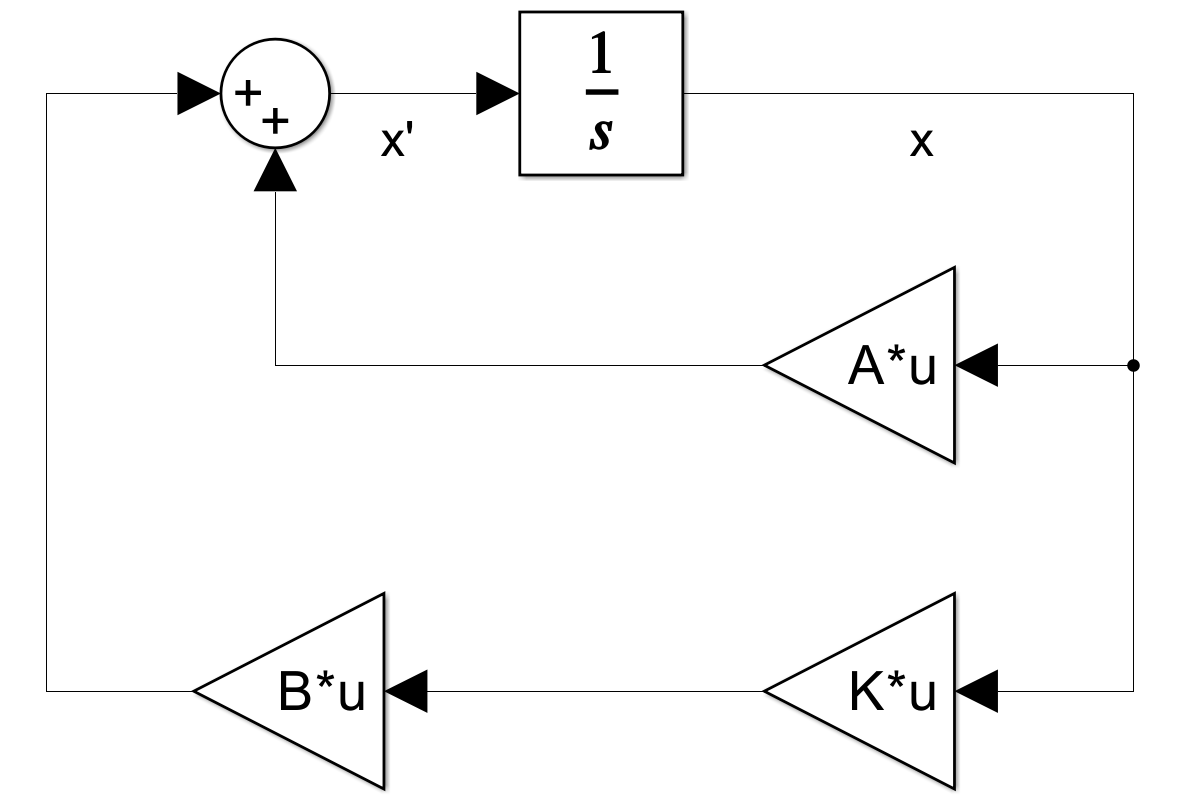
\includegraphics[width=0.7\linewidth]{figs/1_slx.png}
    \caption{Схема моделирования системы \ref{eq:sys1}, замкнутой
    регулятором вида $u=Kx$}
    \label{fig:sys1}
\end{figure}

\subsection{Синтез регулятора}

Зададимся значениями матриц $Q^*\succ0$ и $R^*\succ0$:
\begin{equation*}
    Q^*=\begin{bmatrix}
        1 & 0 & 0\\
        0 & 1 & 0\\
        0 & 0 & 1
    \end{bmatrix},
    R^*=1,
\end{equation*}
и значением параметра $\alpha=1000$, сформируем четыре набора пар матриц $(Q,\ R)$:
$$(Q,\ R),\quad (\alpha Q,\ R),\quad (Q,\ \alpha R),\quad (\alpha Q,\ \alpha R).$$
Для каждой пары $(Q,\ R)$ синтезируем регулятор, минимизируя следующий функционал:
\begin{equation}
    \label{eq:cost1}
    J=\int_0^{\infty}(x^TQx+u^TRu)\ dt,
\end{equation}
путем решения  соответствующего матричного уравнения Риккати:
\begin{equation}
    \label{eq:ric1}
    A^TP+PA-PBR^{-1}B^TP+Q=0,\quad K=-R^{-1}B^TP.
\end{equation}

\subsubsection{Первая пара}

Синтезируем регулятор для первой пары $(Q,\ R)$, используя \texttt{vpasolve}
получим
\begin{equation*}
    K=\begin{bmatrix}
        -1.5798 &  -1.3778  & -7.1171
    \end{bmatrix}.
\end{equation*}
Cоответствующее минимизированное значение функционала качества
\begin{equation*}
    J_{min}=x_0^TPx_0=14.1748,
\end{equation*}
где $P$ - решение соответствующего матричного уравнения Риккати \eqref{eq:ric1}.
Выполним компьютерное моделирование замкнутой системы,
график управления $u(t)$, вектор состояния замкнутой системы $x(t)$ и 
экспериментального значения функционала качества $J_{exp}(t)$ \eqref{eq:cost1}
приведены на \autoref{fig:syssim1}. Для сравнения, $J_{exp}$ установилось на
значении $14.1845$, что очень схоже с $J_{min}$.

\begin{figure}[H]
    \centering
    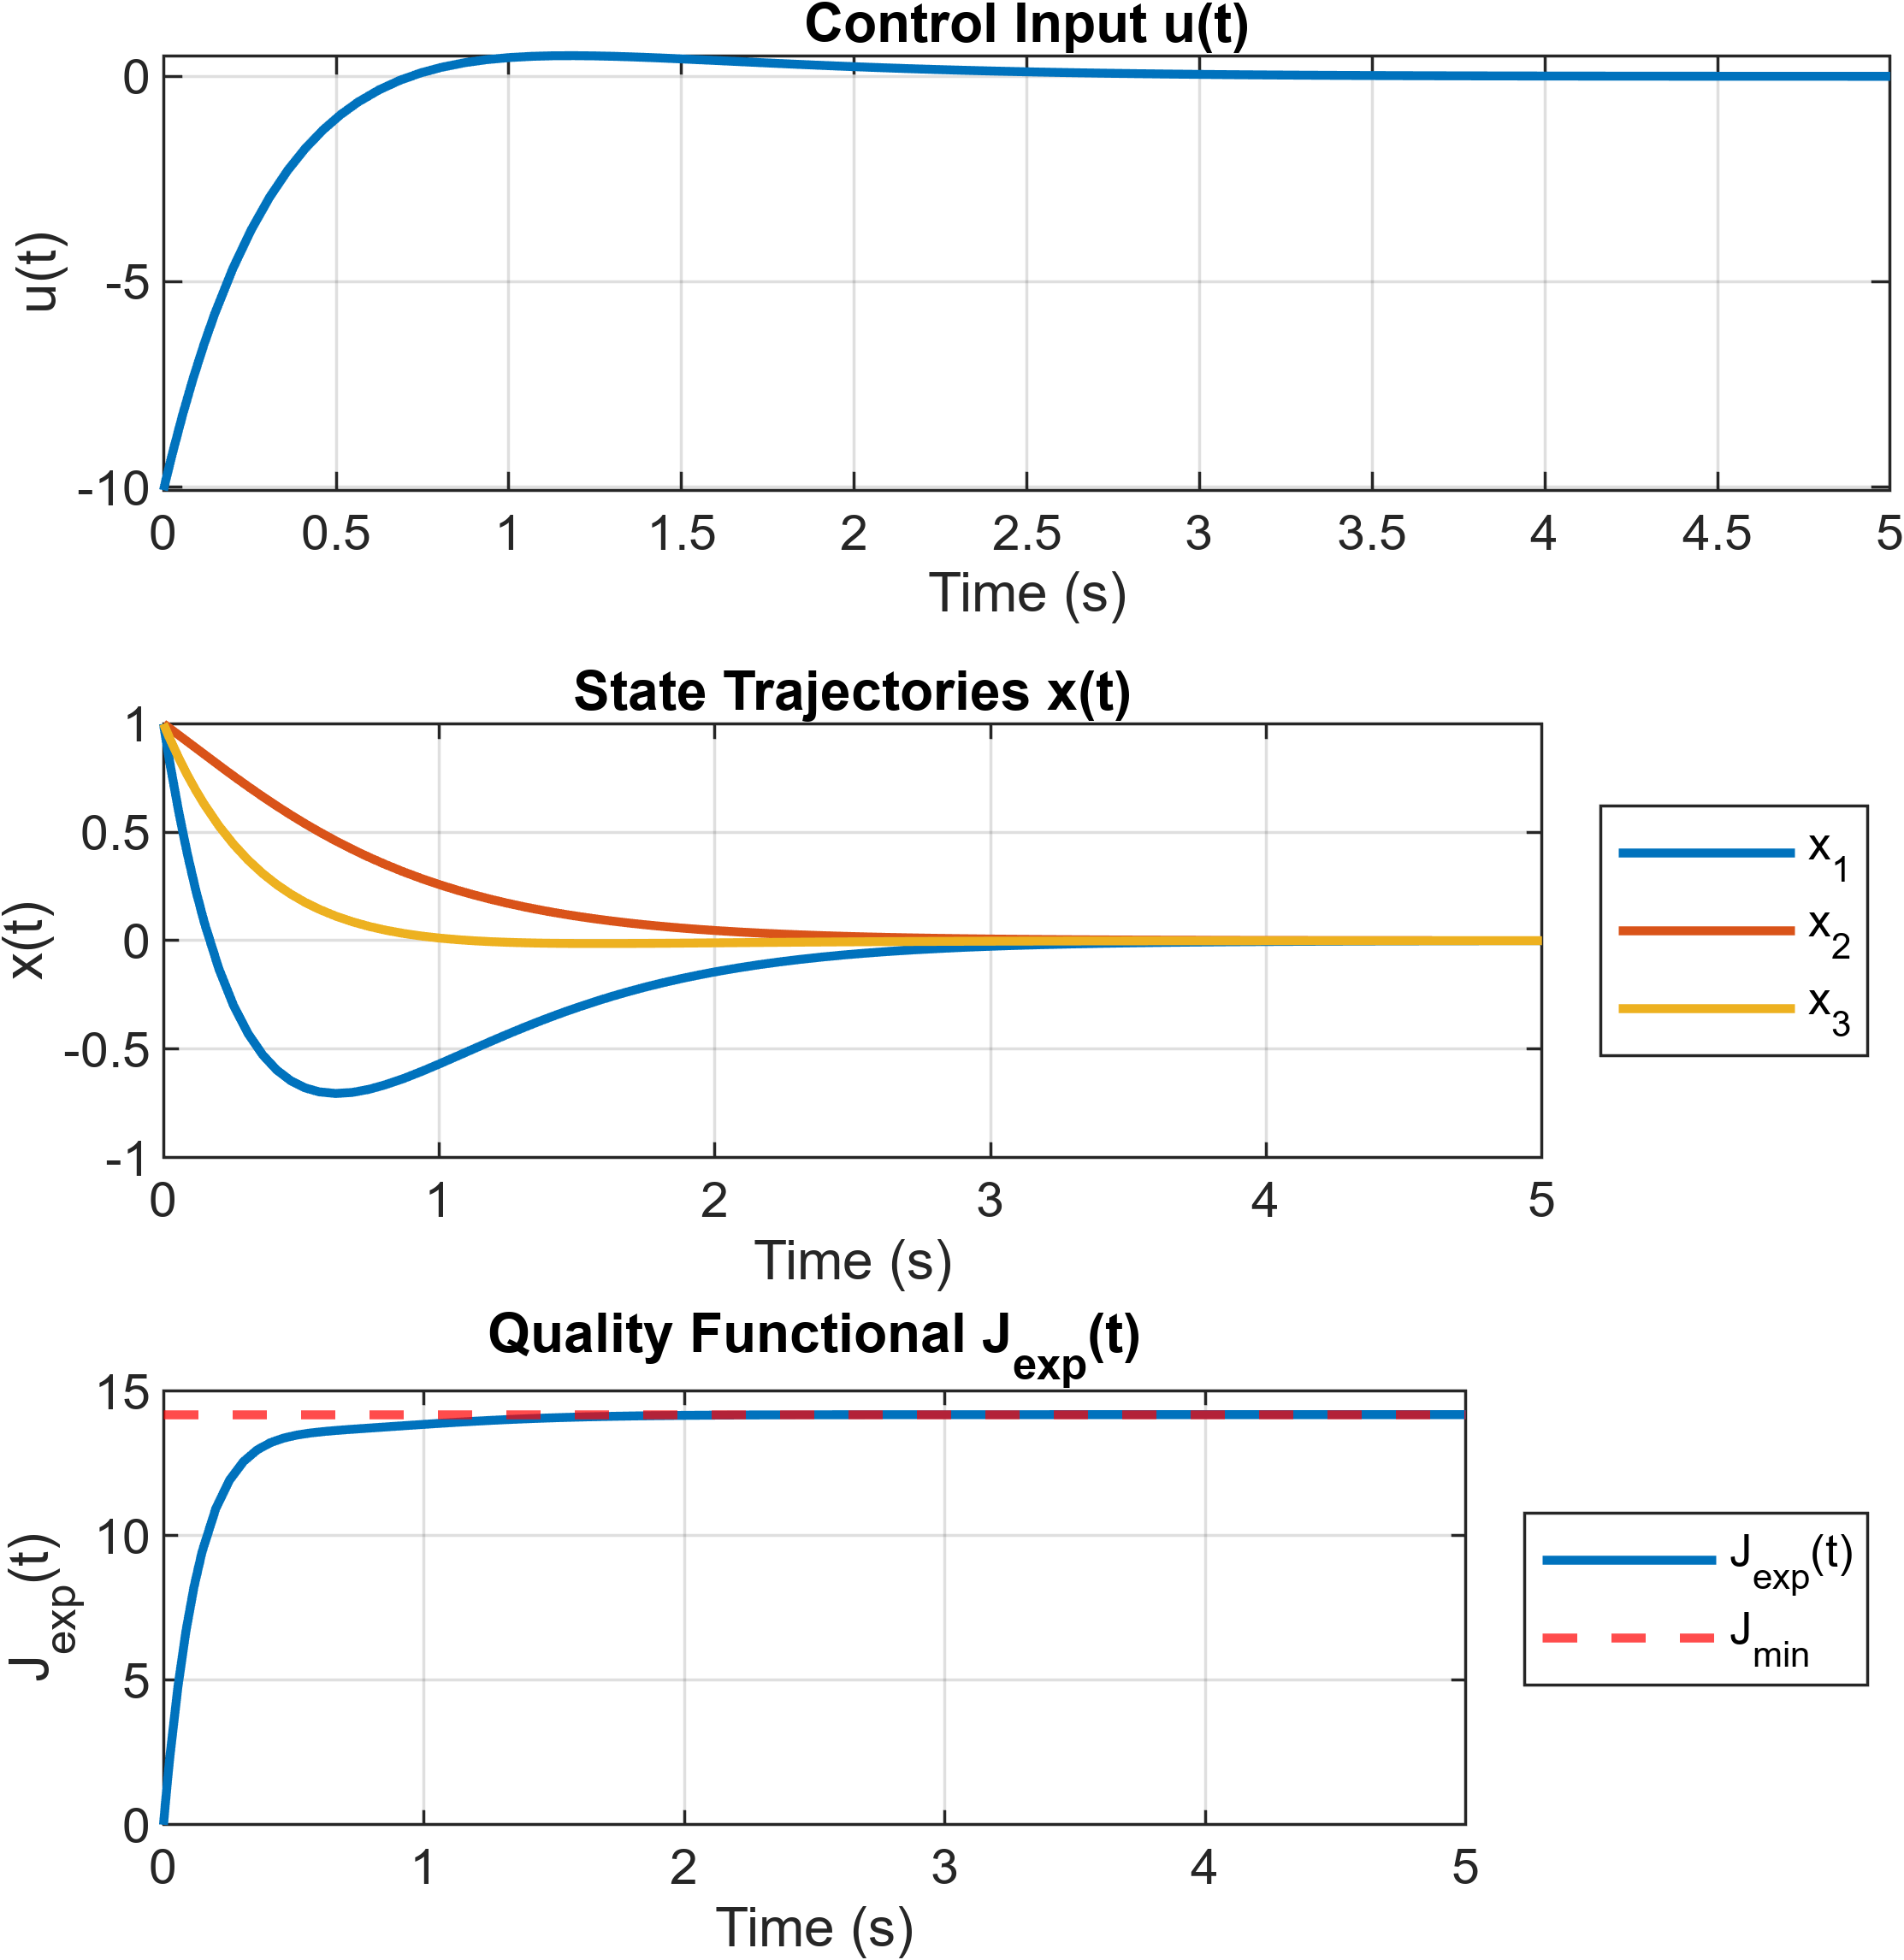
\includegraphics[width=0.9\linewidth]{figs/1_sim1.png}
    \caption{Моделирование замкнутой системы \eqref{eq:sys1} для пары $(Q,\ R)$}
    \label{fig:syssim1}
\end{figure}

\subsubsection{Вторая пара}

Синтезируем регулятор для второй пары $(\alpha Q,\ R)$, используя \texttt{vpasolve}
получим
\begin{equation*}
    K=\begin{bmatrix}
        3.4317  & 18.4307 & -71.2742
    \end{bmatrix}.
\end{equation*}
Cоответствующее минимизированное значение функционала качества
\begin{equation*}
    J_{min}=x_0^TPx_0=836.2982,
\end{equation*}
Выполним компьютерное моделирование замкнутой системы,
результаты приведены на \autoref{fig:syssim2}. Для сравнения, $J_{exp}$ установилось на
значении $836.3231$, что очень схоже с $J_{min}$.


\begin{figure}[H]
    \centering
    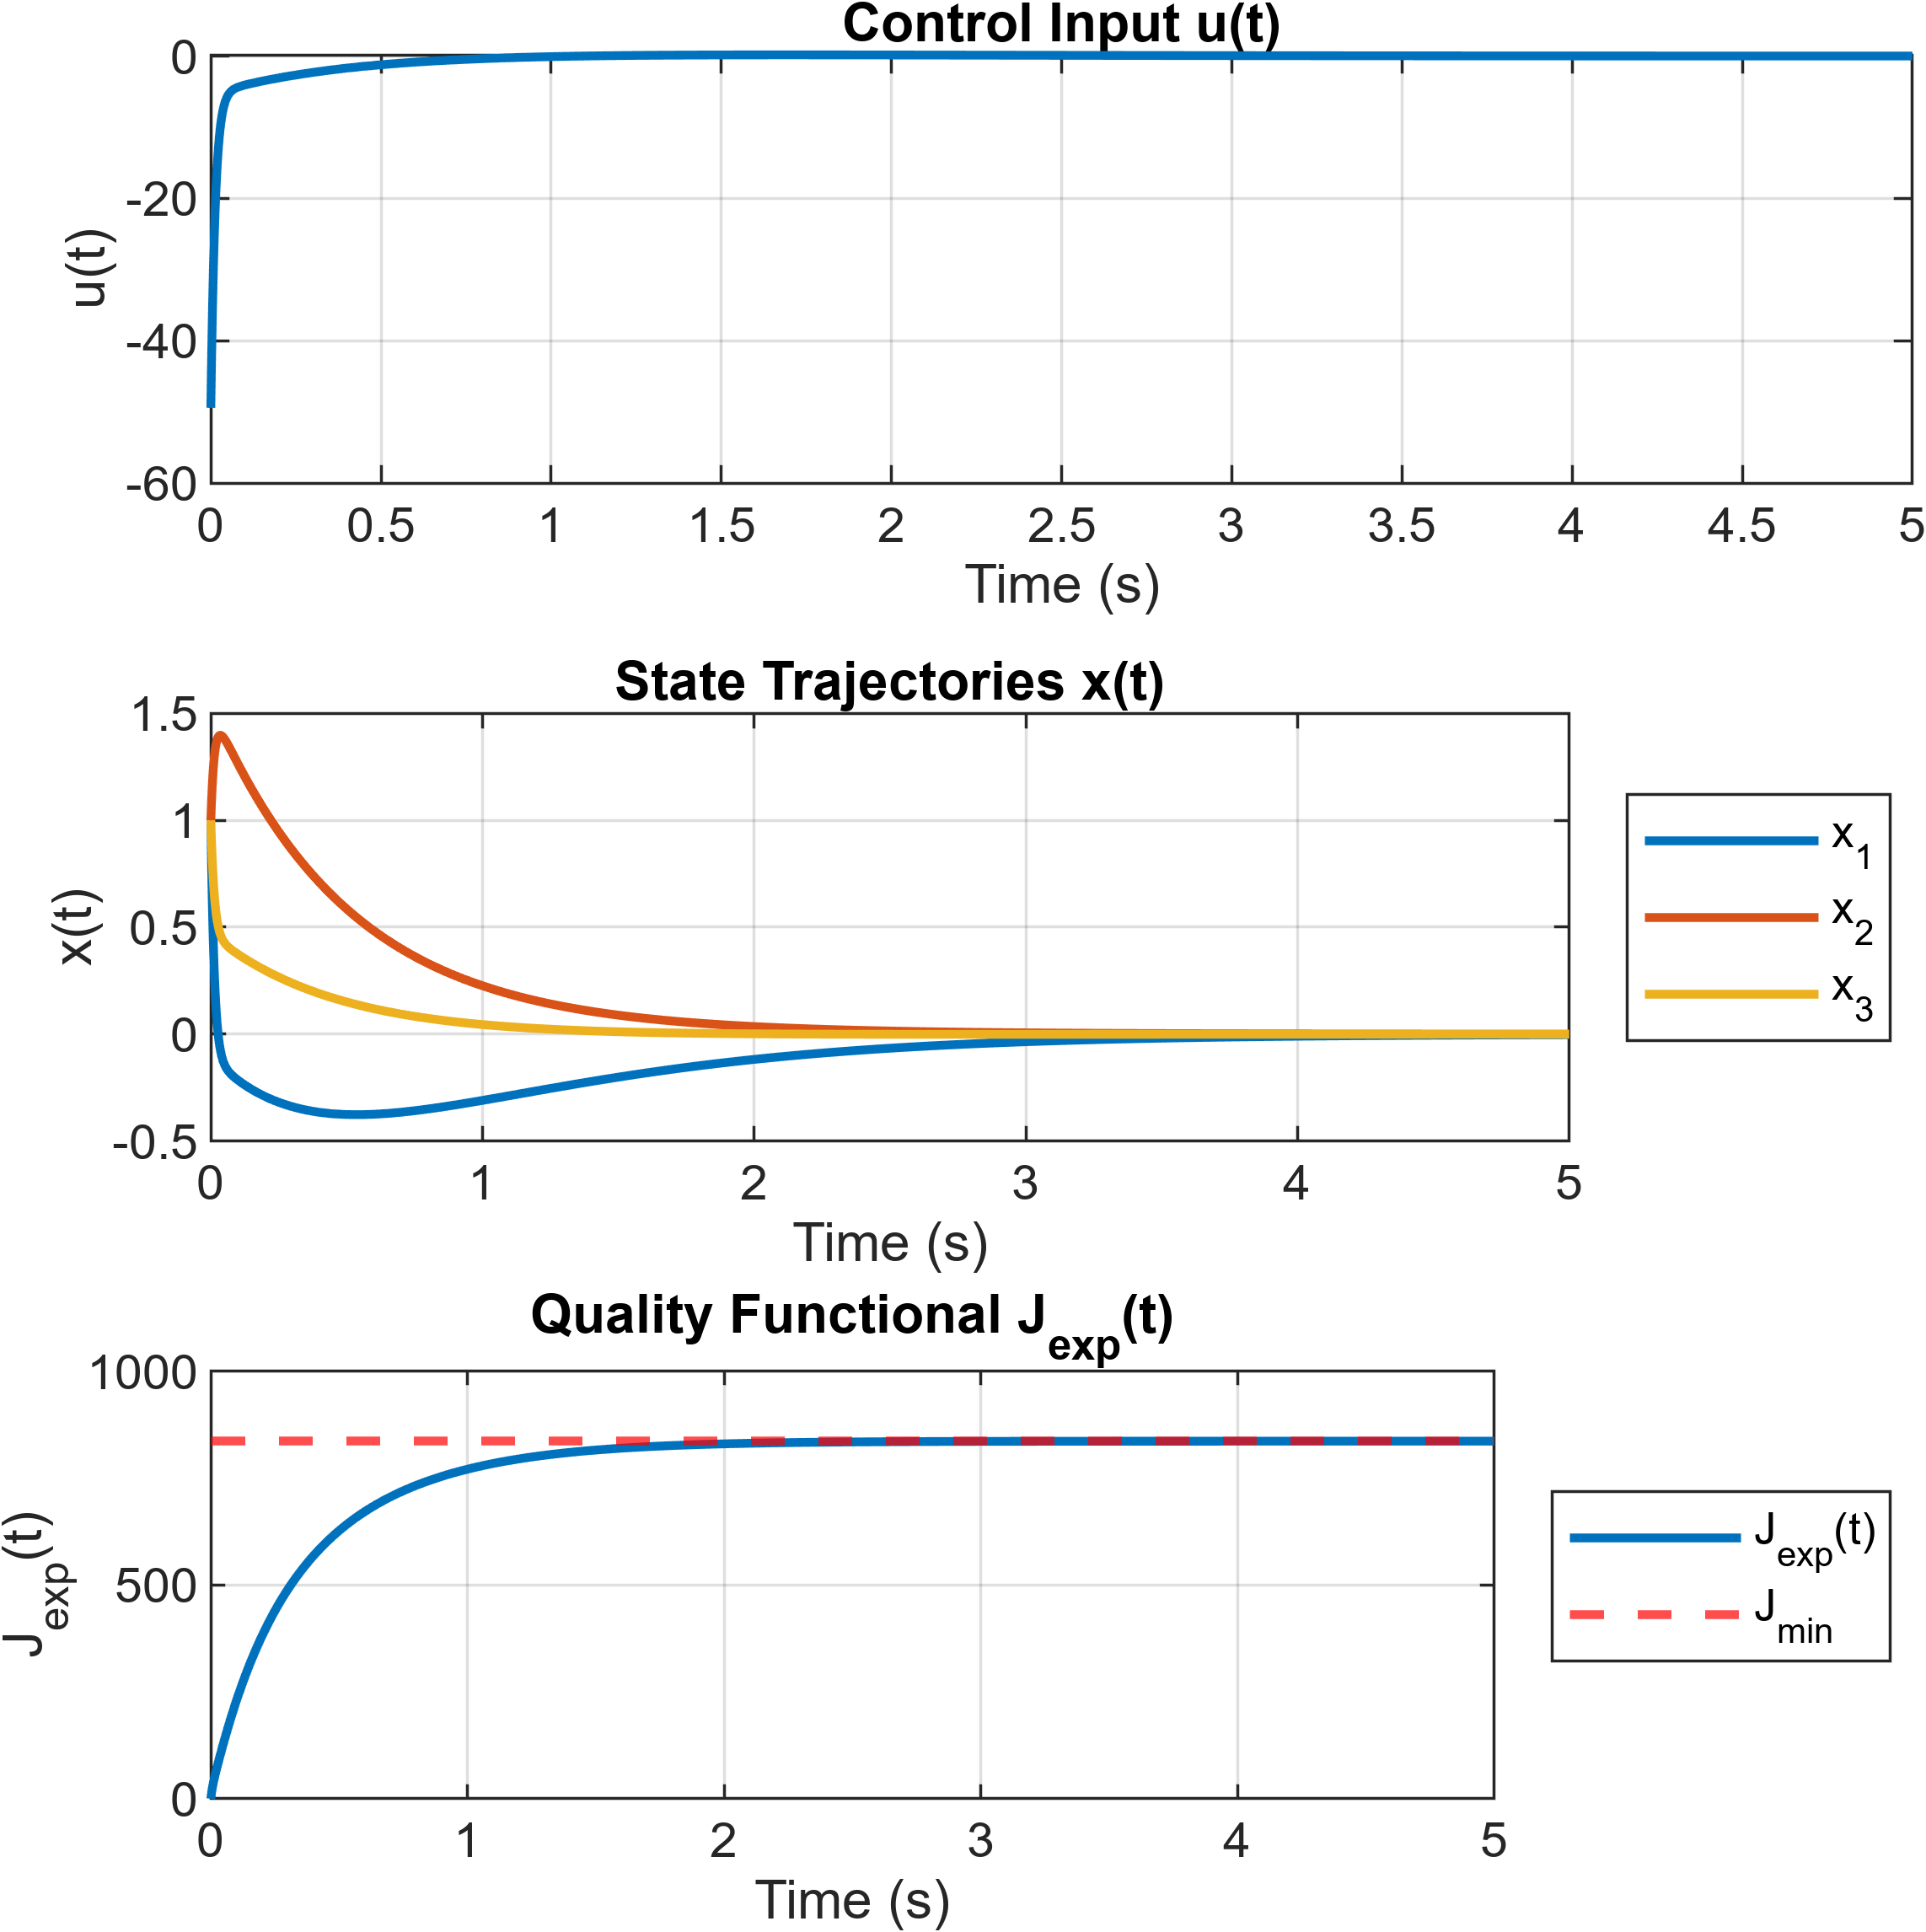
\includegraphics[width=1\linewidth]{figs/1_sim2.png}
    \caption{Моделирование замкнутой системы \eqref{eq:sys1} для пары $(\alpha Q,\ R)$}
    \label{fig:syssim2}
\end{figure}

\subsubsection{Третья пара}

Синтезируем регулятор для третьей пары $(Q,\ \alpha R)$, используя \texttt{vpasolve}
получим
\begin{equation*}
    K=\begin{bmatrix}
        -1.6000  & -1.5997  & -6.4008
    \end{bmatrix}.
\end{equation*}
Cоответствующее минимизированное значение функционала качества
\begin{equation*}
    J_{min}=x_0^TPx_0=13121.0890,
\end{equation*}
Выполним компьютерное моделирование замкнутой системы,
результаты приведены на \autoref{fig:syssim3}. Для сравнения, $J_{exp}$ установилось на
значении $13133$, что очень схоже с $J_{min}$.

\begin{figure}[H]
    \centering
    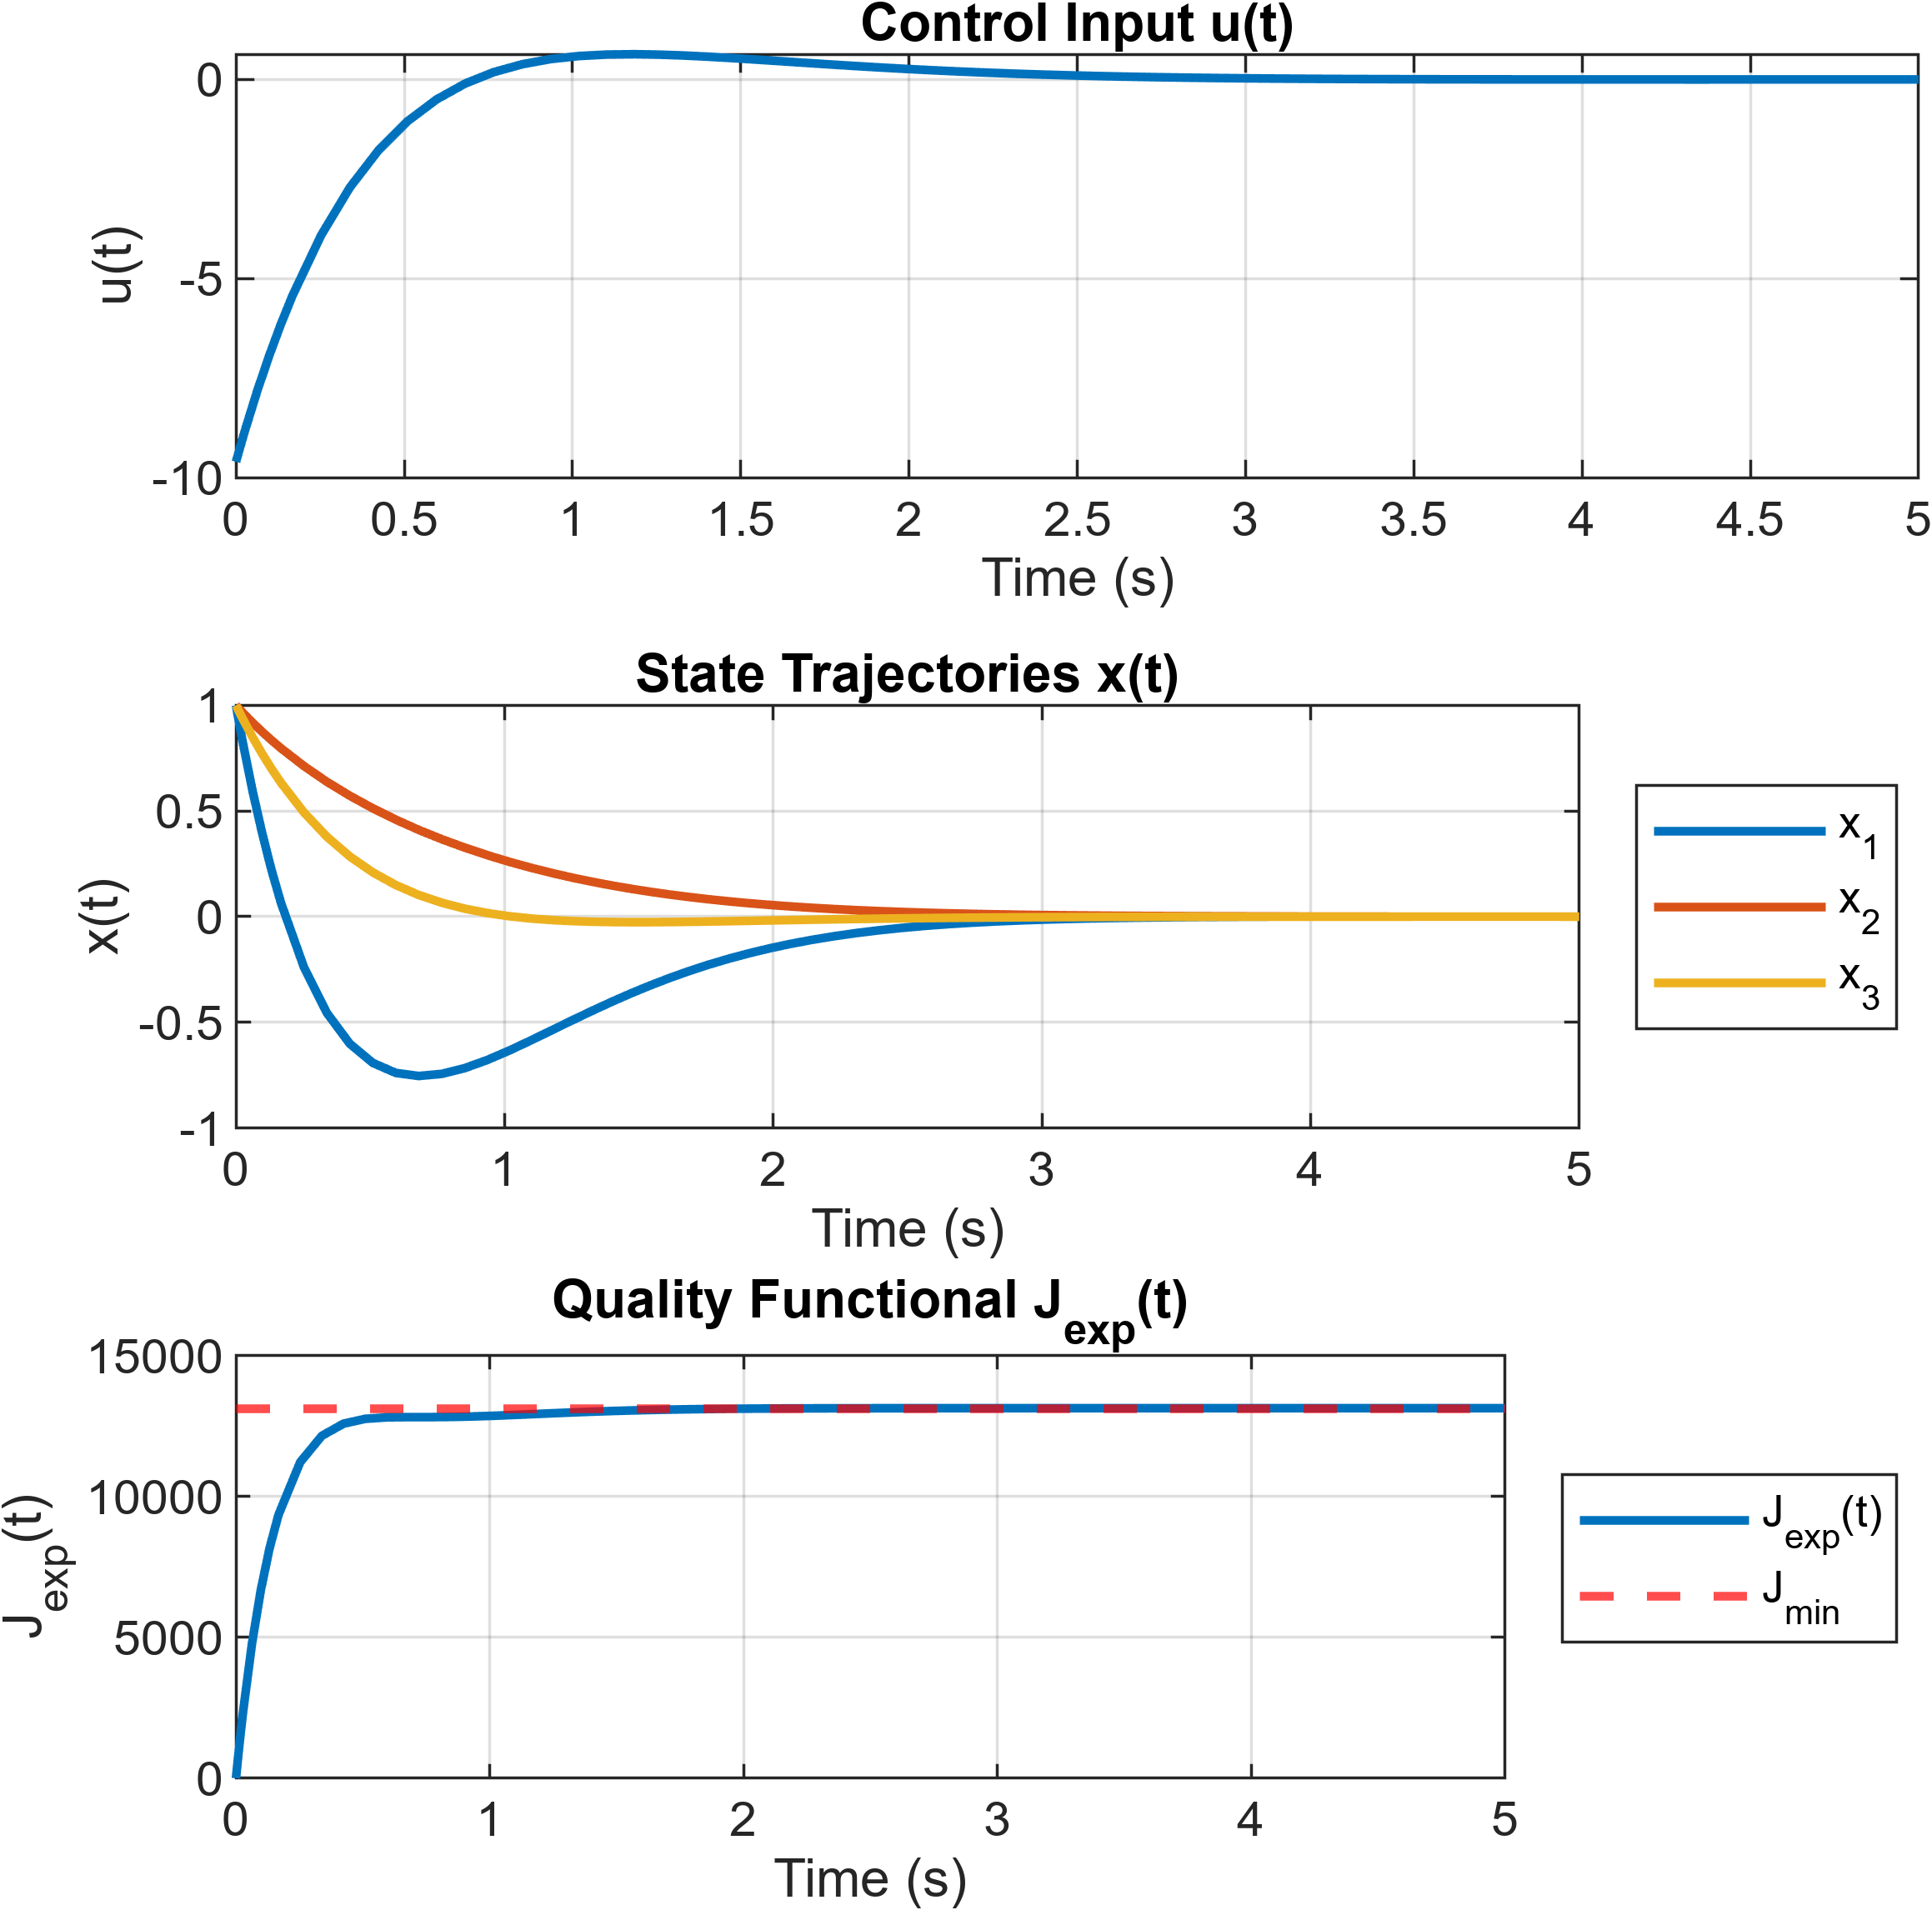
\includegraphics[width=1\linewidth]{figs/1_sim3.png}
    \caption{Моделирование замкнутой системы \eqref{eq:sys1} для пары $(Q,\ \alpha R)$}
    \label{fig:syssim3}
\end{figure}

\newpage\subsubsection{Четвертая пара}

Синтезируем регулятор для четвертой пары $(\alpha Q,\ \alpha R)$, используя \texttt{vpasolve}
получим
\begin{equation*}
    K=\begin{bmatrix}
        -1.5798  & -1.3778 &  -7.1171
    \end{bmatrix}.
\end{equation*}
Cоответствующее минимизированное значение функционала качества
\begin{equation*}
    J_{min}=x_0^TPx_0=14174.7696,
\end{equation*}
Выполним компьютерное моделирование замкнутой системы,
результаты приведены на \autoref{fig:syssim4}. Для сравнения, $J_{exp}$ установилось на
значении $14184$, что очень схоже с $J_{min}$.

\begin{figure}[H]
    \centering
    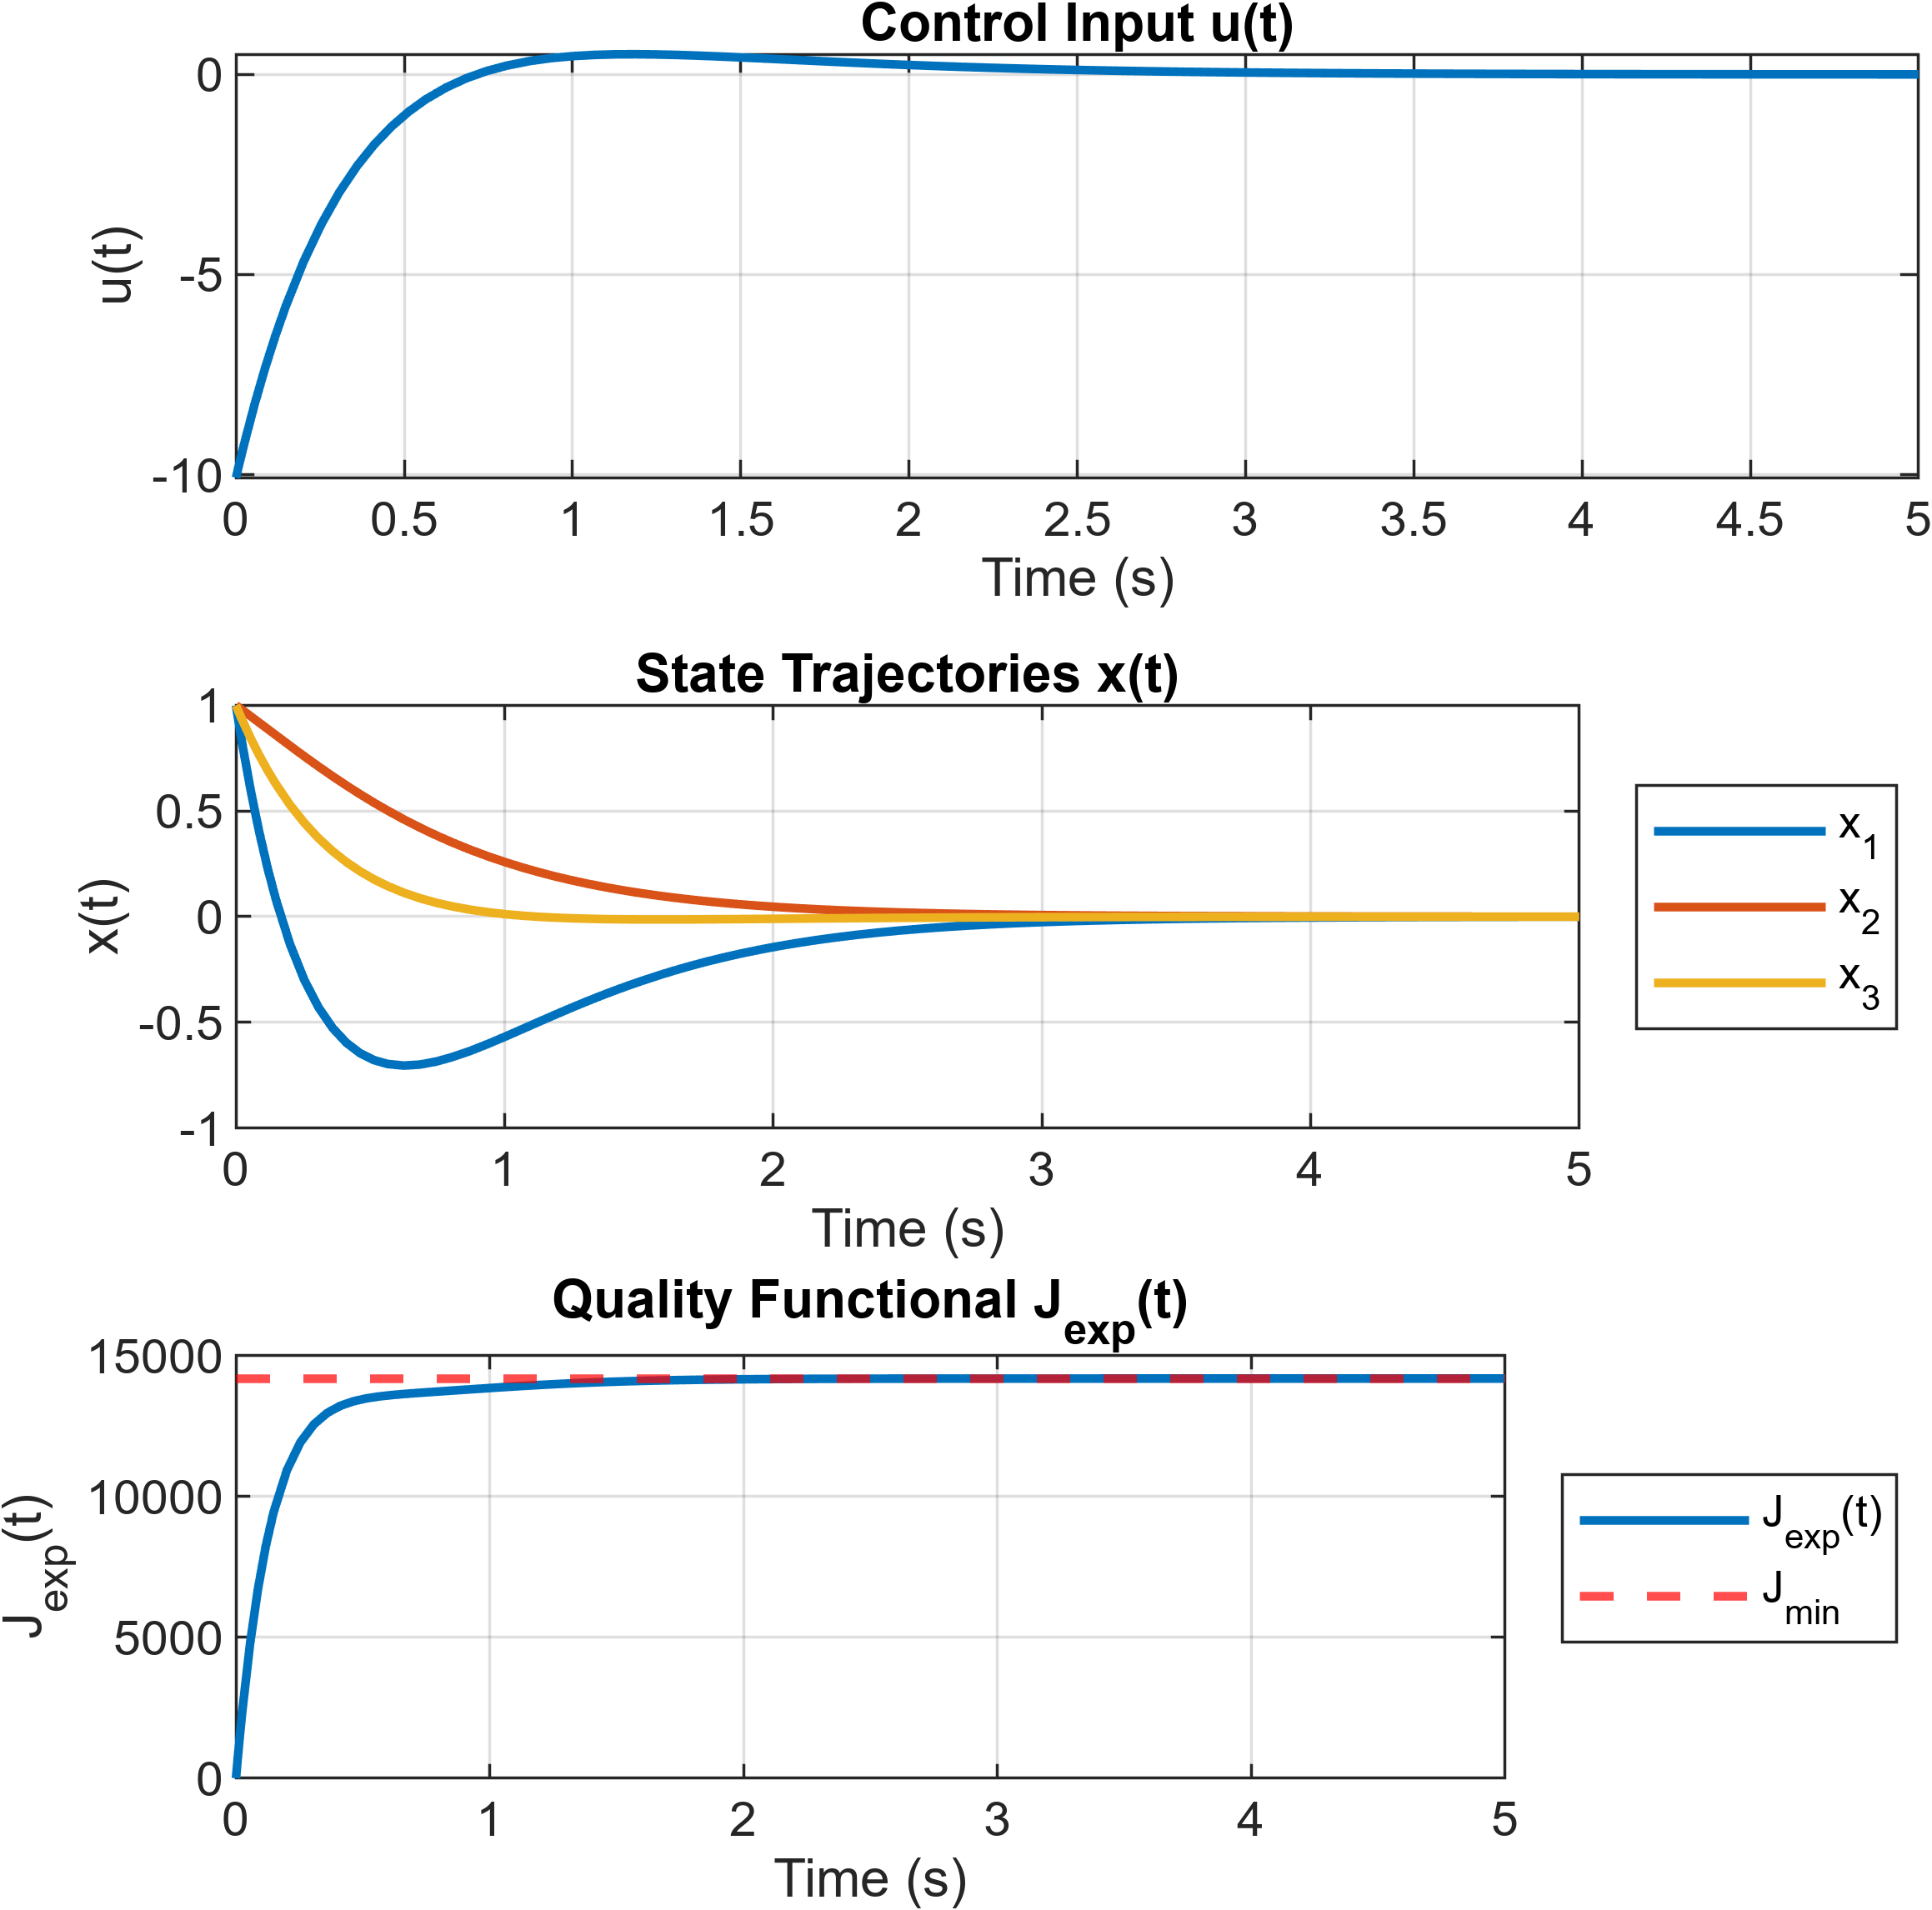
\includegraphics[width=1\linewidth]{figs/1_sim4.png}
    \caption{Моделирование замкнутой системы \eqref{eq:sys1} для пары $(\alpha Q,\ \alpha R)$}
    \label{fig:syssim4}
\end{figure}

\newpage\subsection{Выводы}
Рассмотрев результаты моделирования для различных пар $(Q, R)$, можно сделать 
следующие выводы:
\begin{enumerate}
    \item Увеличение матрицы $Q$ (переход от $(Q, R)$ к $(\alpha Q, R)$) 
    приводит к более агрессивному управлению. Состояние системы пытается
    быстрее сойтись в ноль.
    \item Увеличение матрицы $R$ (переход от $(Q, R)$ к $(Q, \alpha R)$) 
    должно приводить к более мягкому управлению, но, судя по графикам, оно особо не меняется,
    впринципе, управление уже достаточно маленькое, замечу, что
    модуль суммы чисел матрицы управления $K$ уменьшился с $10.0747$ до $9.6005$,
    это говорит об уменьшении управления.
    \item Увеличение обеих матриц $Q$ и $R$ (переход от $(Q, R)$ к $(\alpha Q, \alpha R)$) 
    дает абсолютно никакого эффекта, кроме увеличения значения
    функционала качества $J_{min}$, матрица управления $K$ осталась такой же.
    Это говорит о том, что важно соотношение матриц $Q$ и $R$, а не их
    абсолютные значения.
\end{enumerate}
Таким образом, если элементы $Q$ больше $R$ управление становится более агрессивным, а 
если наоборот — более мягким, обратным образом должно изменяться и скорость сходимости
состояния, но в данном моделировании это плохо видно, что можно заметить, так это
менее гладкие графики состояния, при более агрессивном управлении.





\newpage \section{Исследование фильтра Калмана}
\subsection{Система}
Рассмотрим систему:
\begin{equation}
    \label{eq:sys2}
    \begin{cases}
        \dot x=Ax+f\\
        y=Cx+\xi
    \end{cases},\quad
    x(0)=\begin{bmatrix}
        1&1&1&1
    \end{bmatrix}^T,
\end{equation}
где $f(t)$ и $\xi(t)$ - гайссовский белый шум,
\begin{equation*}
    A=\begin{bmatrix}
        25 & 8 & -20 & 13 \\
        -38 & -11 & 30 & -18 \\
        40 & 13 & -33 & 21 \\
        38 & 12 & -32 & 19
        \end{bmatrix},\quad
        C=\begin{bmatrix}
        7 & 2 & -5 & 3
        \end{bmatrix}.
\end{equation*}
Используя матрицу наблюдаемости:
\begin{equation*}
    V=\begin{bmatrix}
        7 & 2 & -5 & 3 \\
        13 & 5 & -11 & 7 \\
        -39 & -10 & 29 & -19 \\
        -157 & -53 & 131 & -79
    \end{bmatrix},
\end{equation*}
понимаем, что система \eqref{eq:sys2} наблюдаема, так как ранг матрицы $V$ равен 4,
как следствие система и обнаруживаема.
Построим структурную схему системы \eqref{eq:sys2} с наблюдателем состояния
$\dot{\hat x}=A\hat x+L(C\hat x-y)$, см. \autoref{fig:sys2}.
\begin{figure}[H]
    \centering
    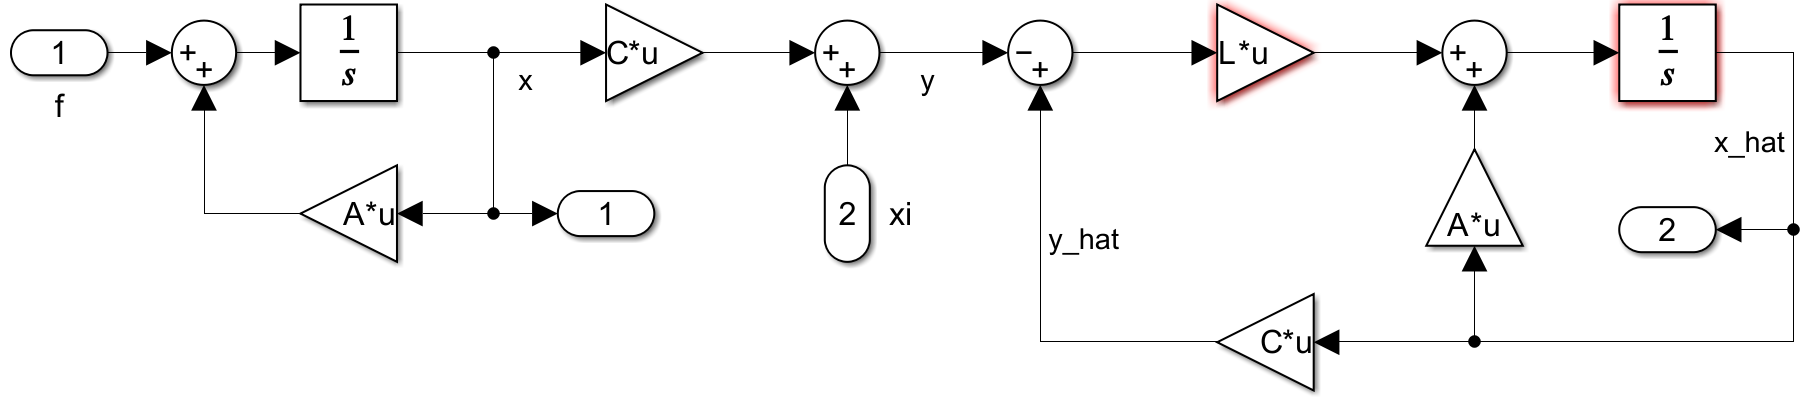
\includegraphics[width=1\linewidth]{figs/2_slx.png}
    \caption{Схема моделирования системы \eqref{eq:sys2} с наблюдателем состояния}
    \label{fig:sys2}
\end{figure}

\subsection{Синтез регулятора}

Зададимся значениями матриц $Q^*\succ0$ и $R^*\succ0$:
\begin{equation*}
    Q^*=\begin{bmatrix}
        1 & 0 & 0\\
        0 & 1 & 0\\
        0 & 0 & 1
    \end{bmatrix},
    R^*=1,
\end{equation*}
и значением параметра $\alpha=1000$, сформируем четыре набора пар матриц $(Q,\ R)$:
$$(Q,\ R),\quad (\alpha Q,\ R),\quad (Q,\ \alpha R),\quad (\alpha Q,\ \alpha R).$$
Для каждой пары $(Q,\ R)$ синтезируем регулятор, минимизируя следующий функционал:
\begin{equation}
    \label{eq:cost2}
    J=\int_0^{\infty}(f^TQf+\xi^TR\xi)\ dt,
\end{equation}
путем решения  соответствующего матричного уравнения Риккати:
\begin{equation}
    \label{eq:ric2}
    AP+PA^T-PC^TR^{-1}CP+Q=0,\quad L=-PC^TR^{-1}.
\end{equation}

\subsubsection{Первая пара}

Синтезируем наблюдатель для первой пары $(Q,\ R)$, используя \texttt{icare} получим
\begin{equation*}
    L=\begin{bmatrix}
        -2.6323&
        -12.9504&
         -6.7362&
         -0.4351
    \end{bmatrix}^T.
\end{equation*}
Выполним компьютерное моделирование системы с нулевыми начальными условиями
наблюдателя, для воспроизведения гауссовского белого шума будем использовать
функцию \texttt{mvnrnd}, мат. ожидание у обоих сигналов нулевое, дисперсии следующие:
\begin{equation*}
    \sigma_f=\begin{bmatrix}
        1 & 0 & 0 & 0\\
        0 & 1 & 0 & 0\\
        0 & 0 & 1 & 0\\
        0 & 0 & 0 & 1
    \end{bmatrix},\quad
    \sigma_\xi=1.
\end{equation*} 
Сравнительные графики $x(t)$ и $\hat x(t)$, а также
график ошибки $e(t)=\hat x(t)-x(t)$ наблюдателя
приведены на \autoref{fig:sys2sim1}.

\begin{figure}[H]
    \centering
    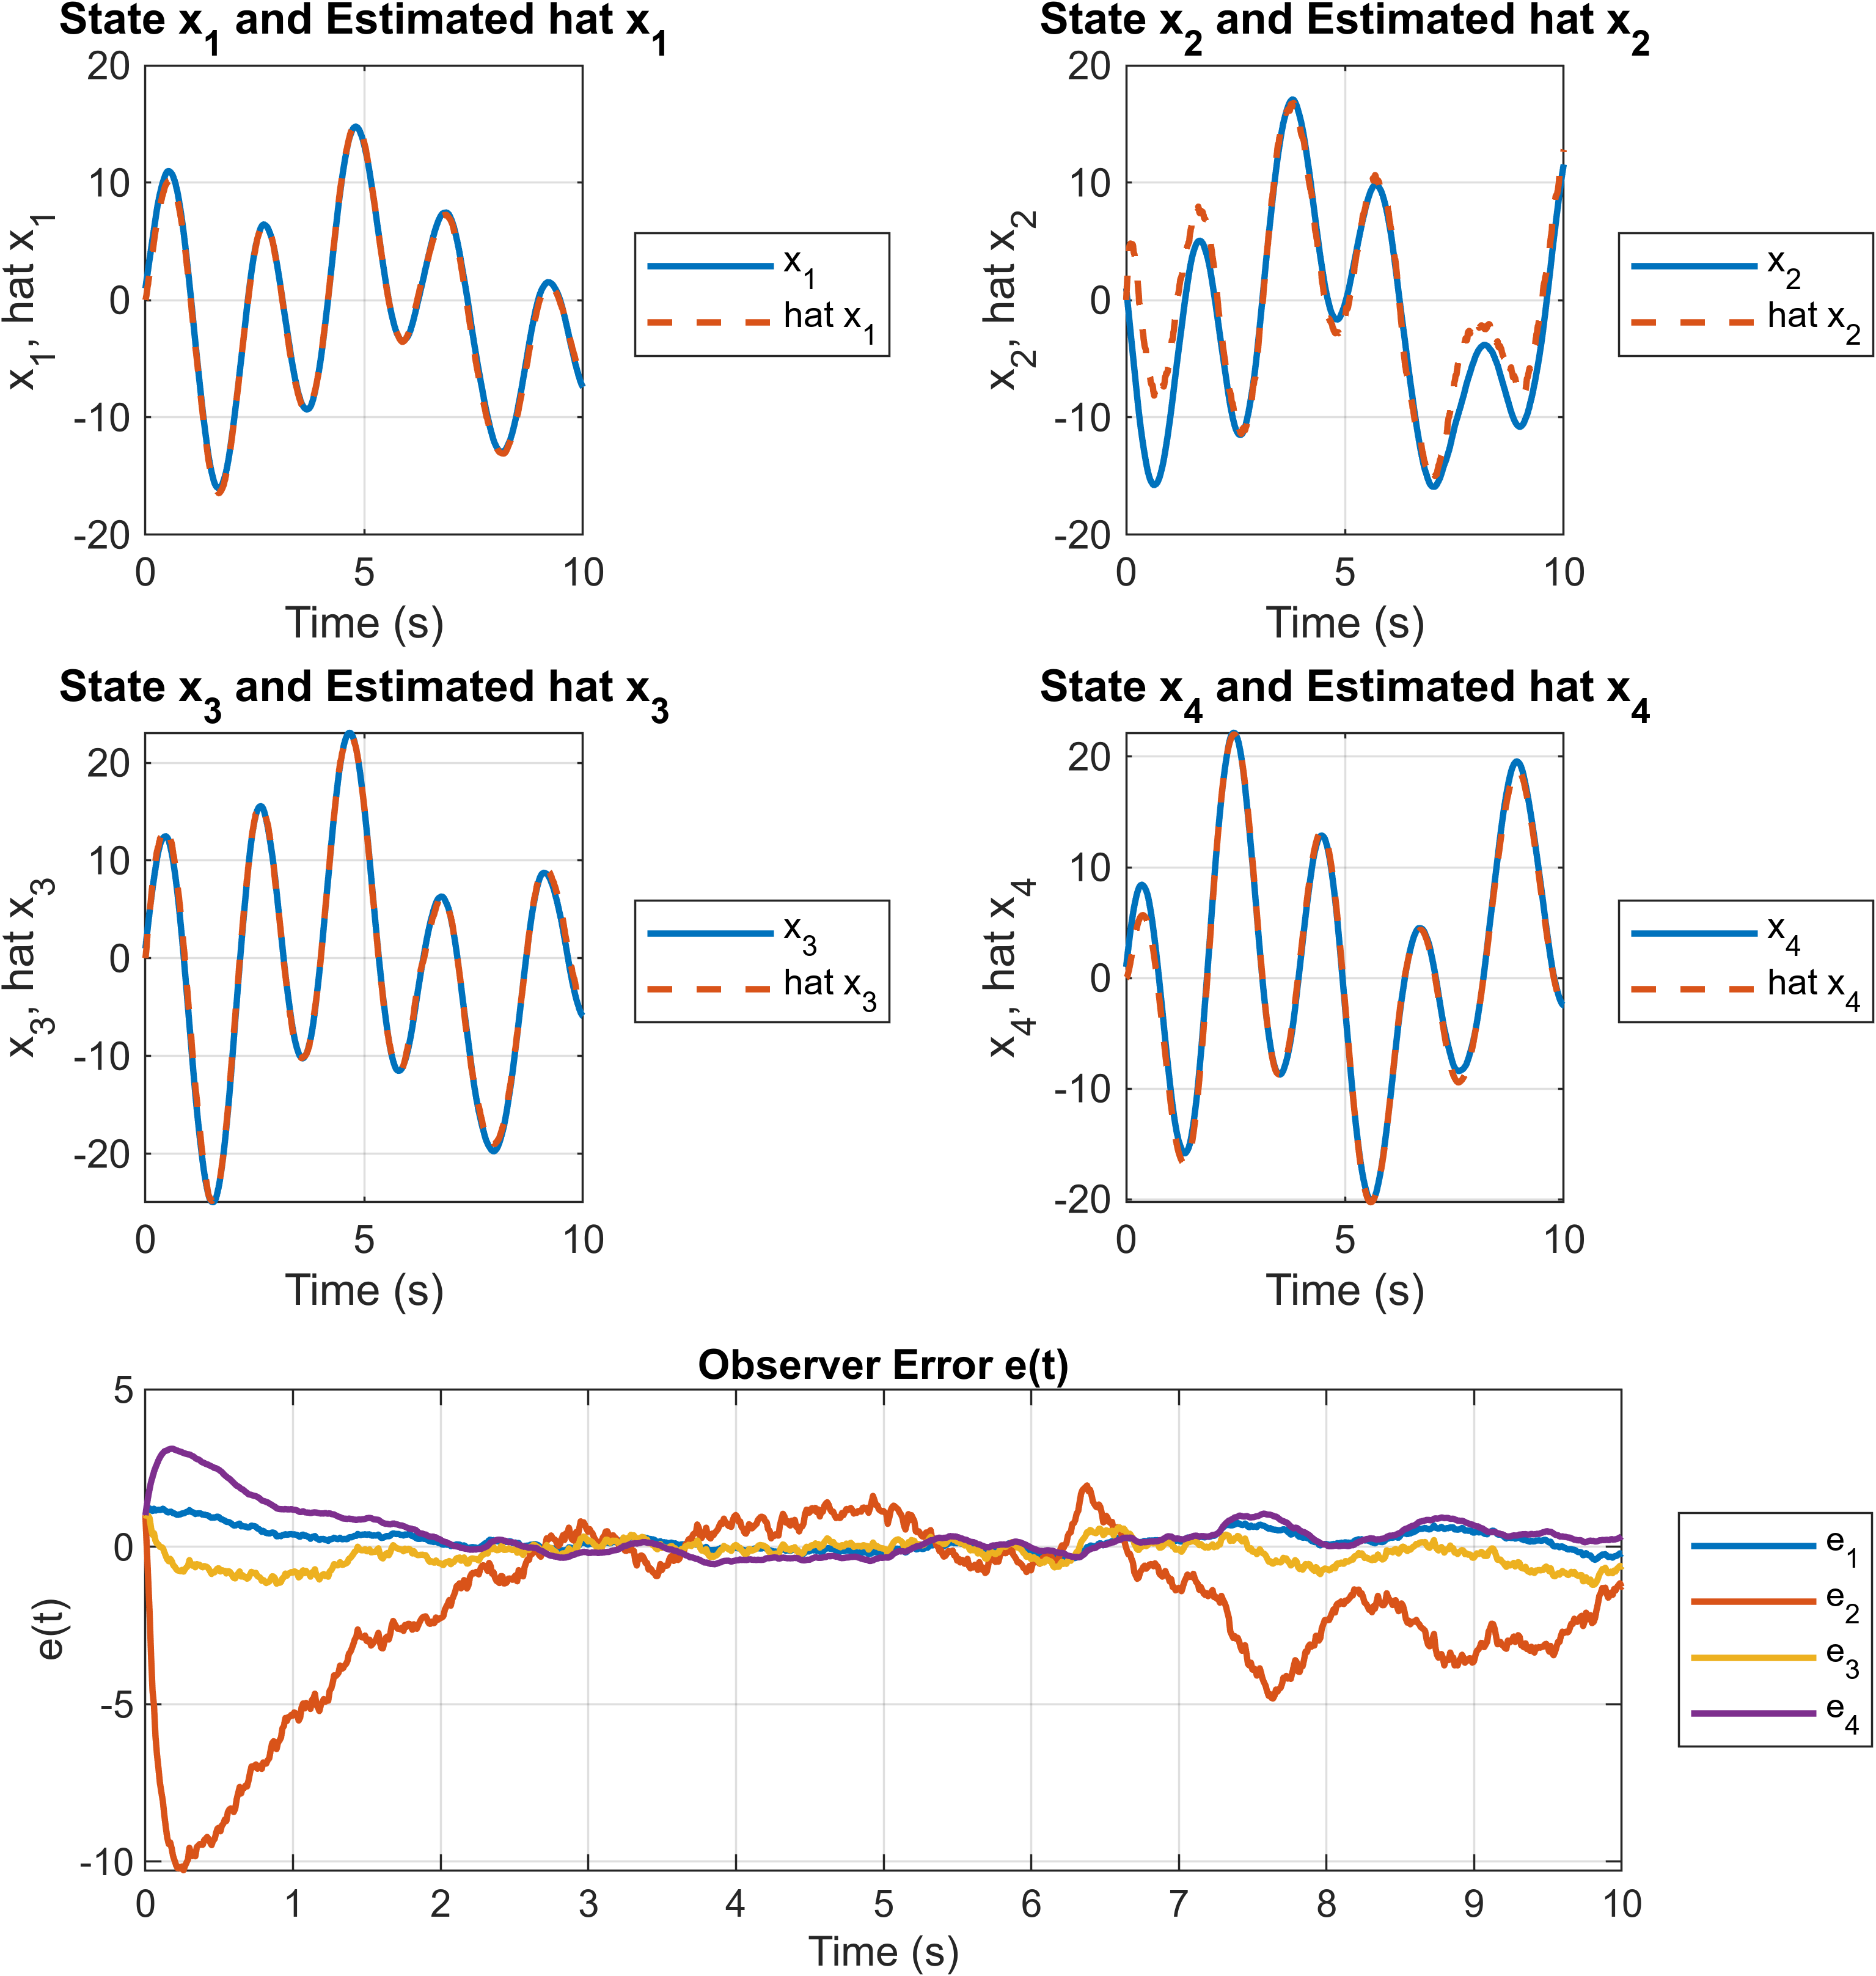
\includegraphics[width=0.9\linewidth]{figs/2_sim1.png}
    \caption{Моделирование замкнутой системы \eqref{eq:sys2} для пары $(Q,\ R)$}
    \label{fig:sys2sim1}
\end{figure}

\newpage\subsubsection{Вторая пара}

Синтезируем наблюдатель для второй пары $(\alpha Q,\ R)$, используя \texttt{icare} получим
\begin{equation*}
    L=\begin{bmatrix}
        20.0527&
        -530.3858&
         -49.4616&
         124.9529
    \end{bmatrix}^T.
\end{equation*}
Выполним компьютерное моделирование системы. Графики приведены на \autoref{fig:sys2sim2}.

\begin{figure}[H]
    \centering
    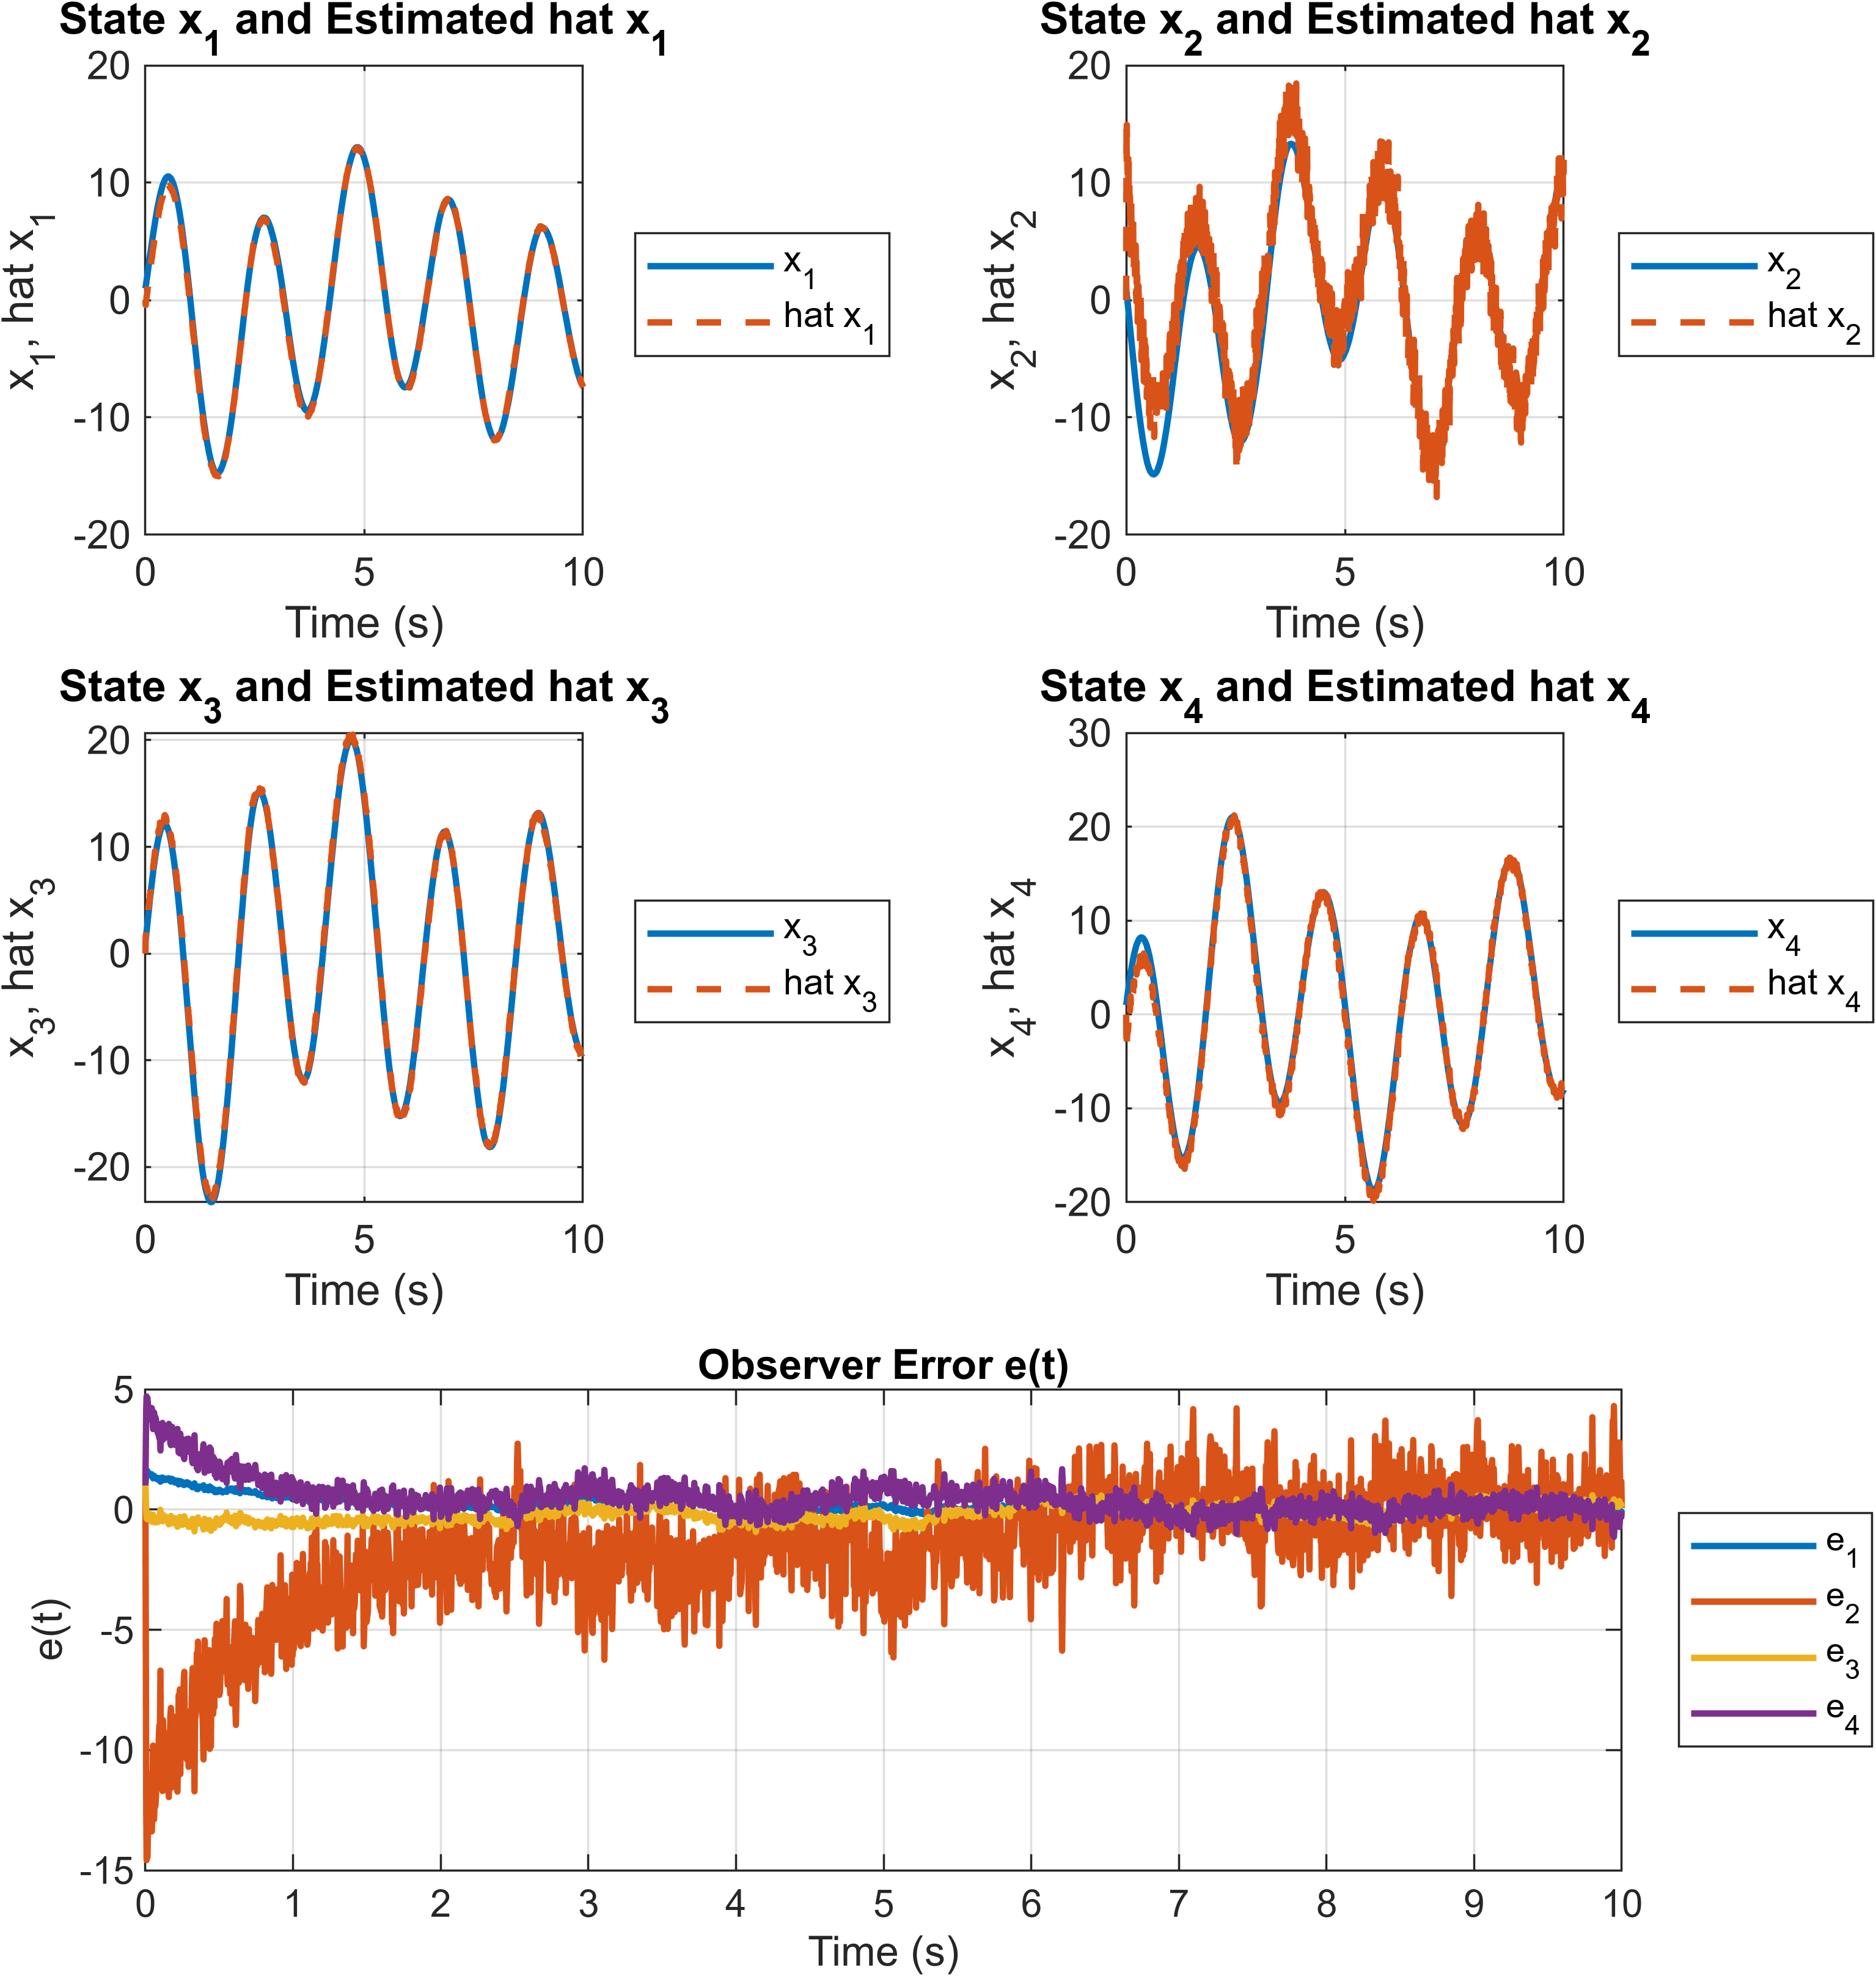
\includegraphics[width=1\linewidth]{figs/2_sim2.png}
    \caption{Моделирование замкнутой системы \eqref{eq:sys2} для пары $(\alpha Q,\ R)$}
    \label{fig:sys2sim2}
\end{figure}

\newpage\subsubsection{Третья пара}

Синтезируем наблюдатель для третей пары $(Q,\ \alpha R)$, используя \texttt{icare} получим
\begin{equation*}
    L=\begin{bmatrix}
        -0.5258&
        0.0379&
       -0.8397&
       -0.3869
    \end{bmatrix}^T.
\end{equation*}
Выполним компьютерное моделирование системы. Графики приведены на \autoref{fig:sys2sim3}.

\begin{figure}[H]
    \centering
    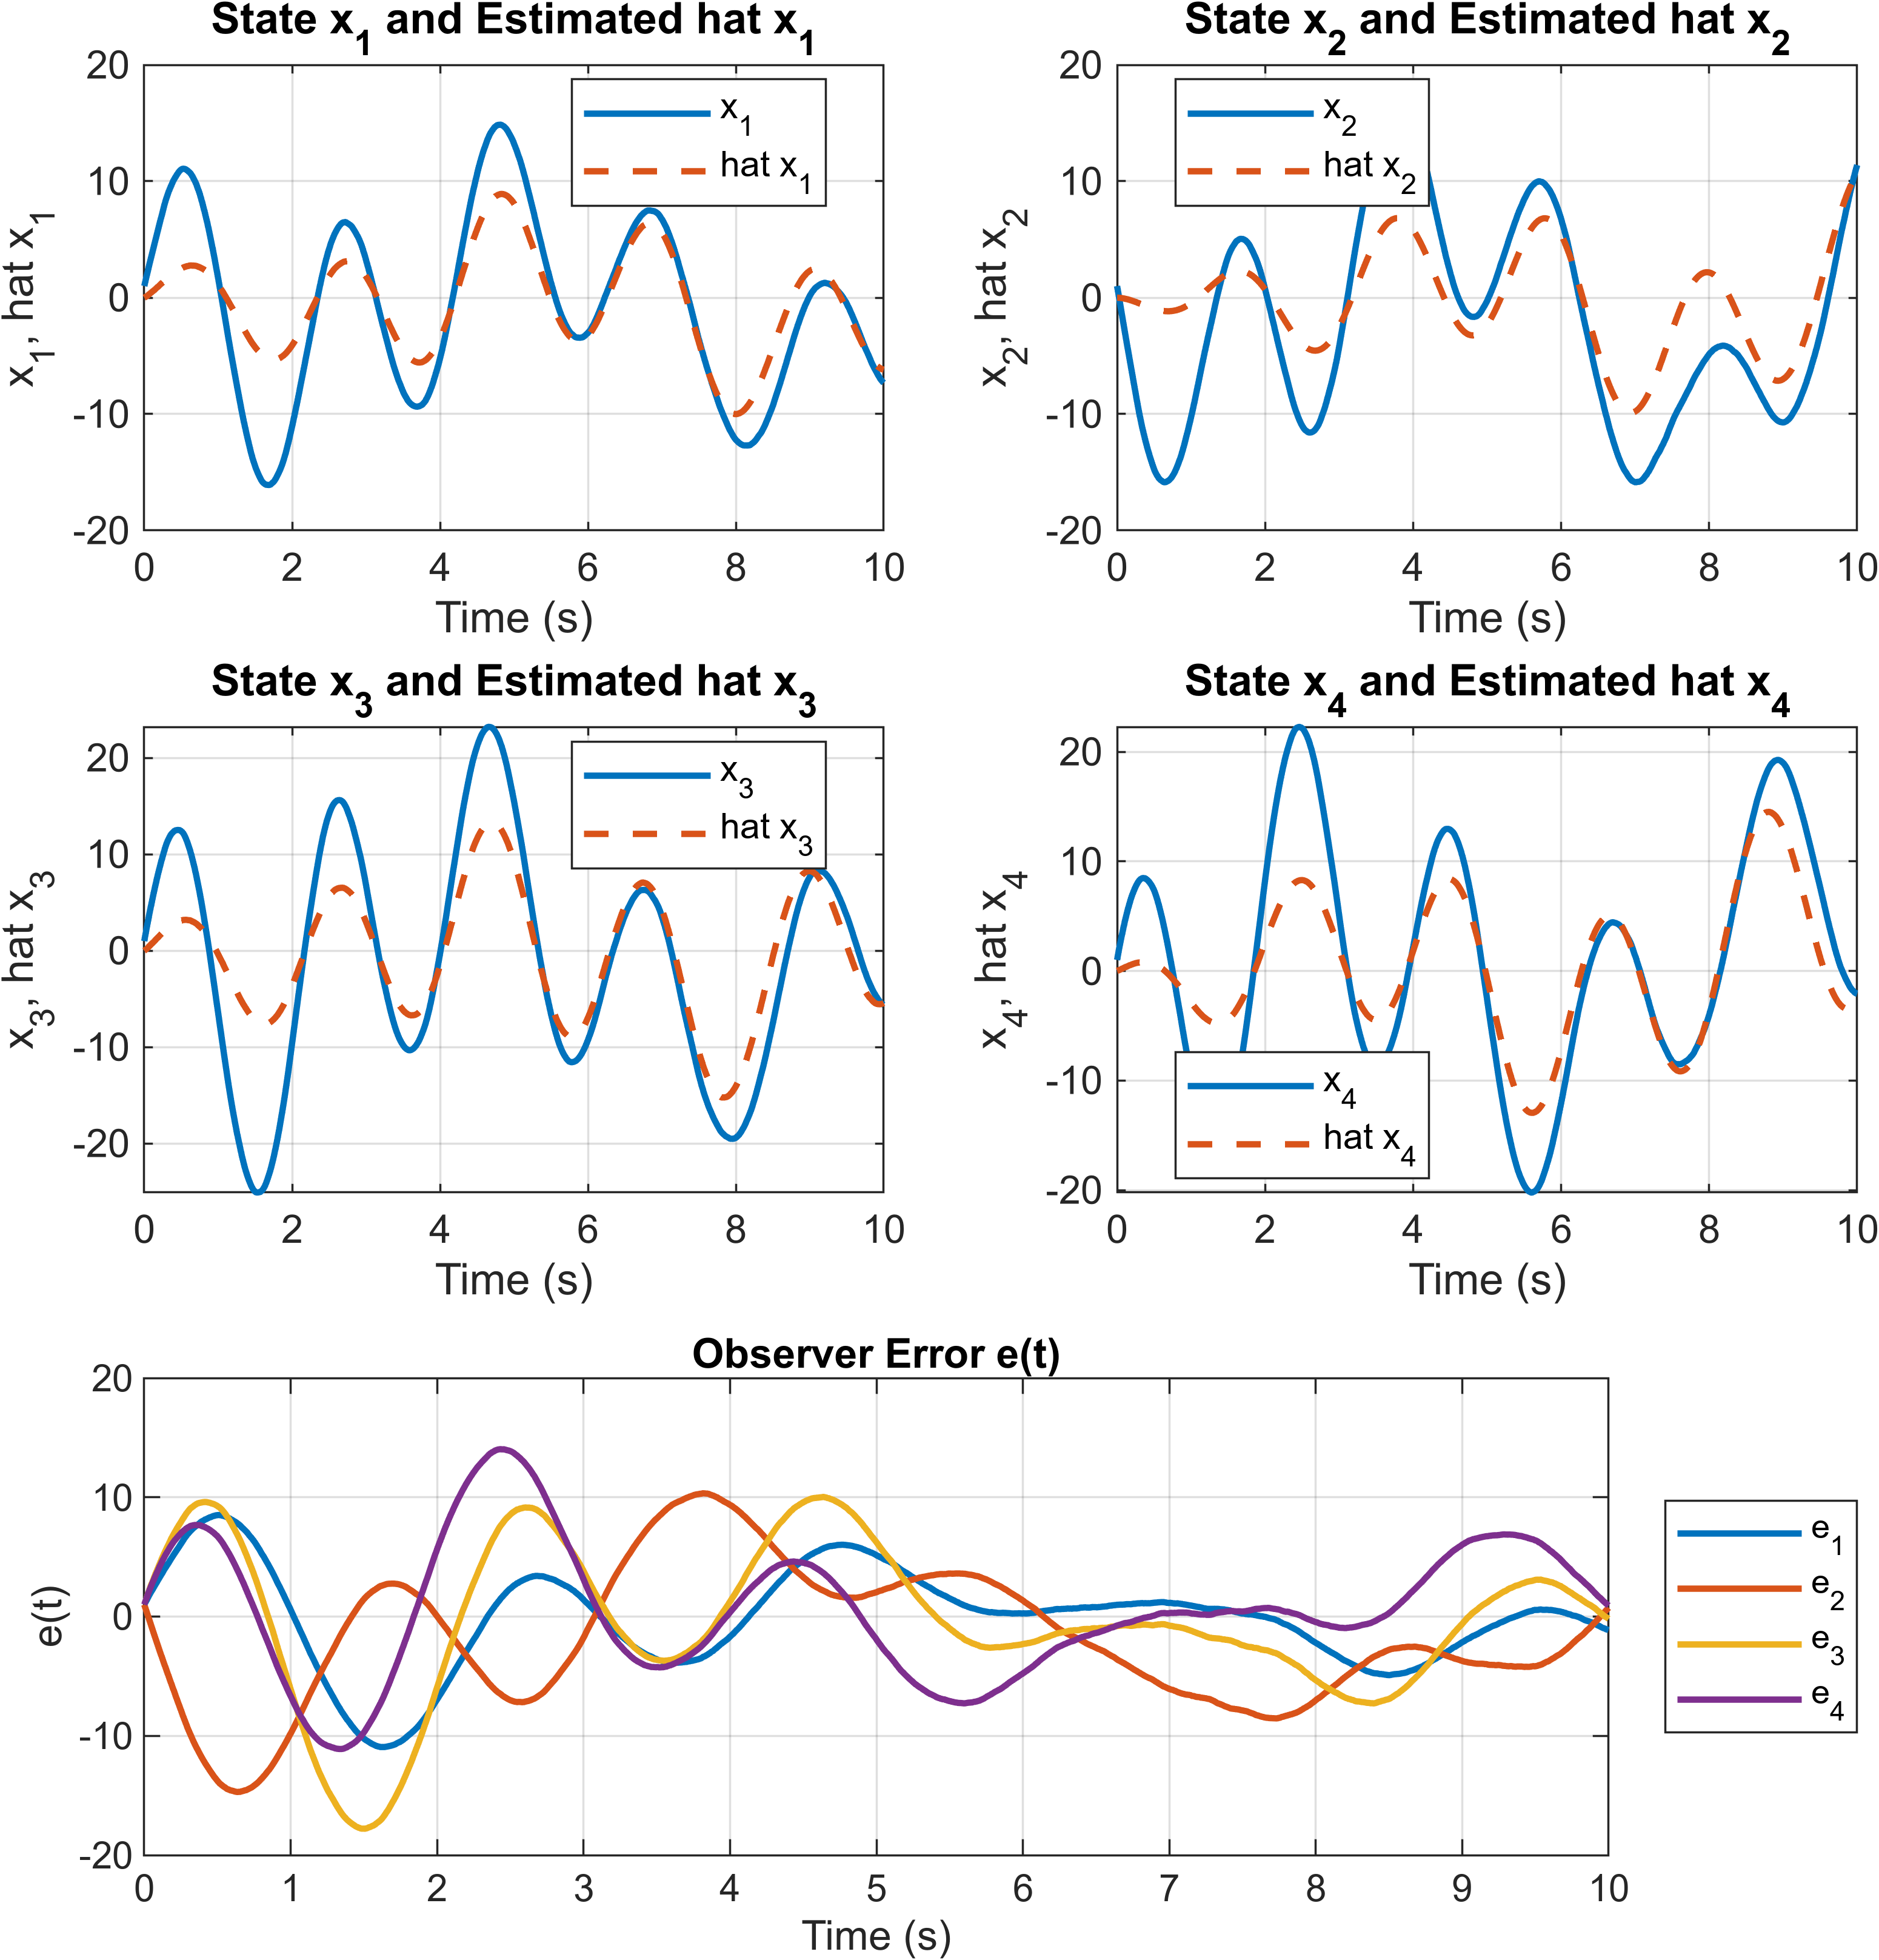
\includegraphics[width=1\linewidth]{figs/2_sim3.png}
    \caption{Моделирование замкнутой системы \eqref{eq:sys2} для пары $(Q,\ \alpha  R )$}
    \label{fig:sys2sim3}
\end{figure}

\newpage\subsubsection{Четвертая пара}

Синтезируем наблюдатель для четвертой пары $(\alpha Q,\ \alpha R)$, используя \texttt{icare} получим
\begin{equation*}
    L=\begin{bmatrix}
        -2.6323&
        -12.9504&
         -6.7362&
         -0.4351
    \end{bmatrix}^T.
\end{equation*}
Выполним компьютерное моделирование системы. Графики приведены на \autoref{fig:sys2sim4}.

\begin{figure}[H]
    \centering
    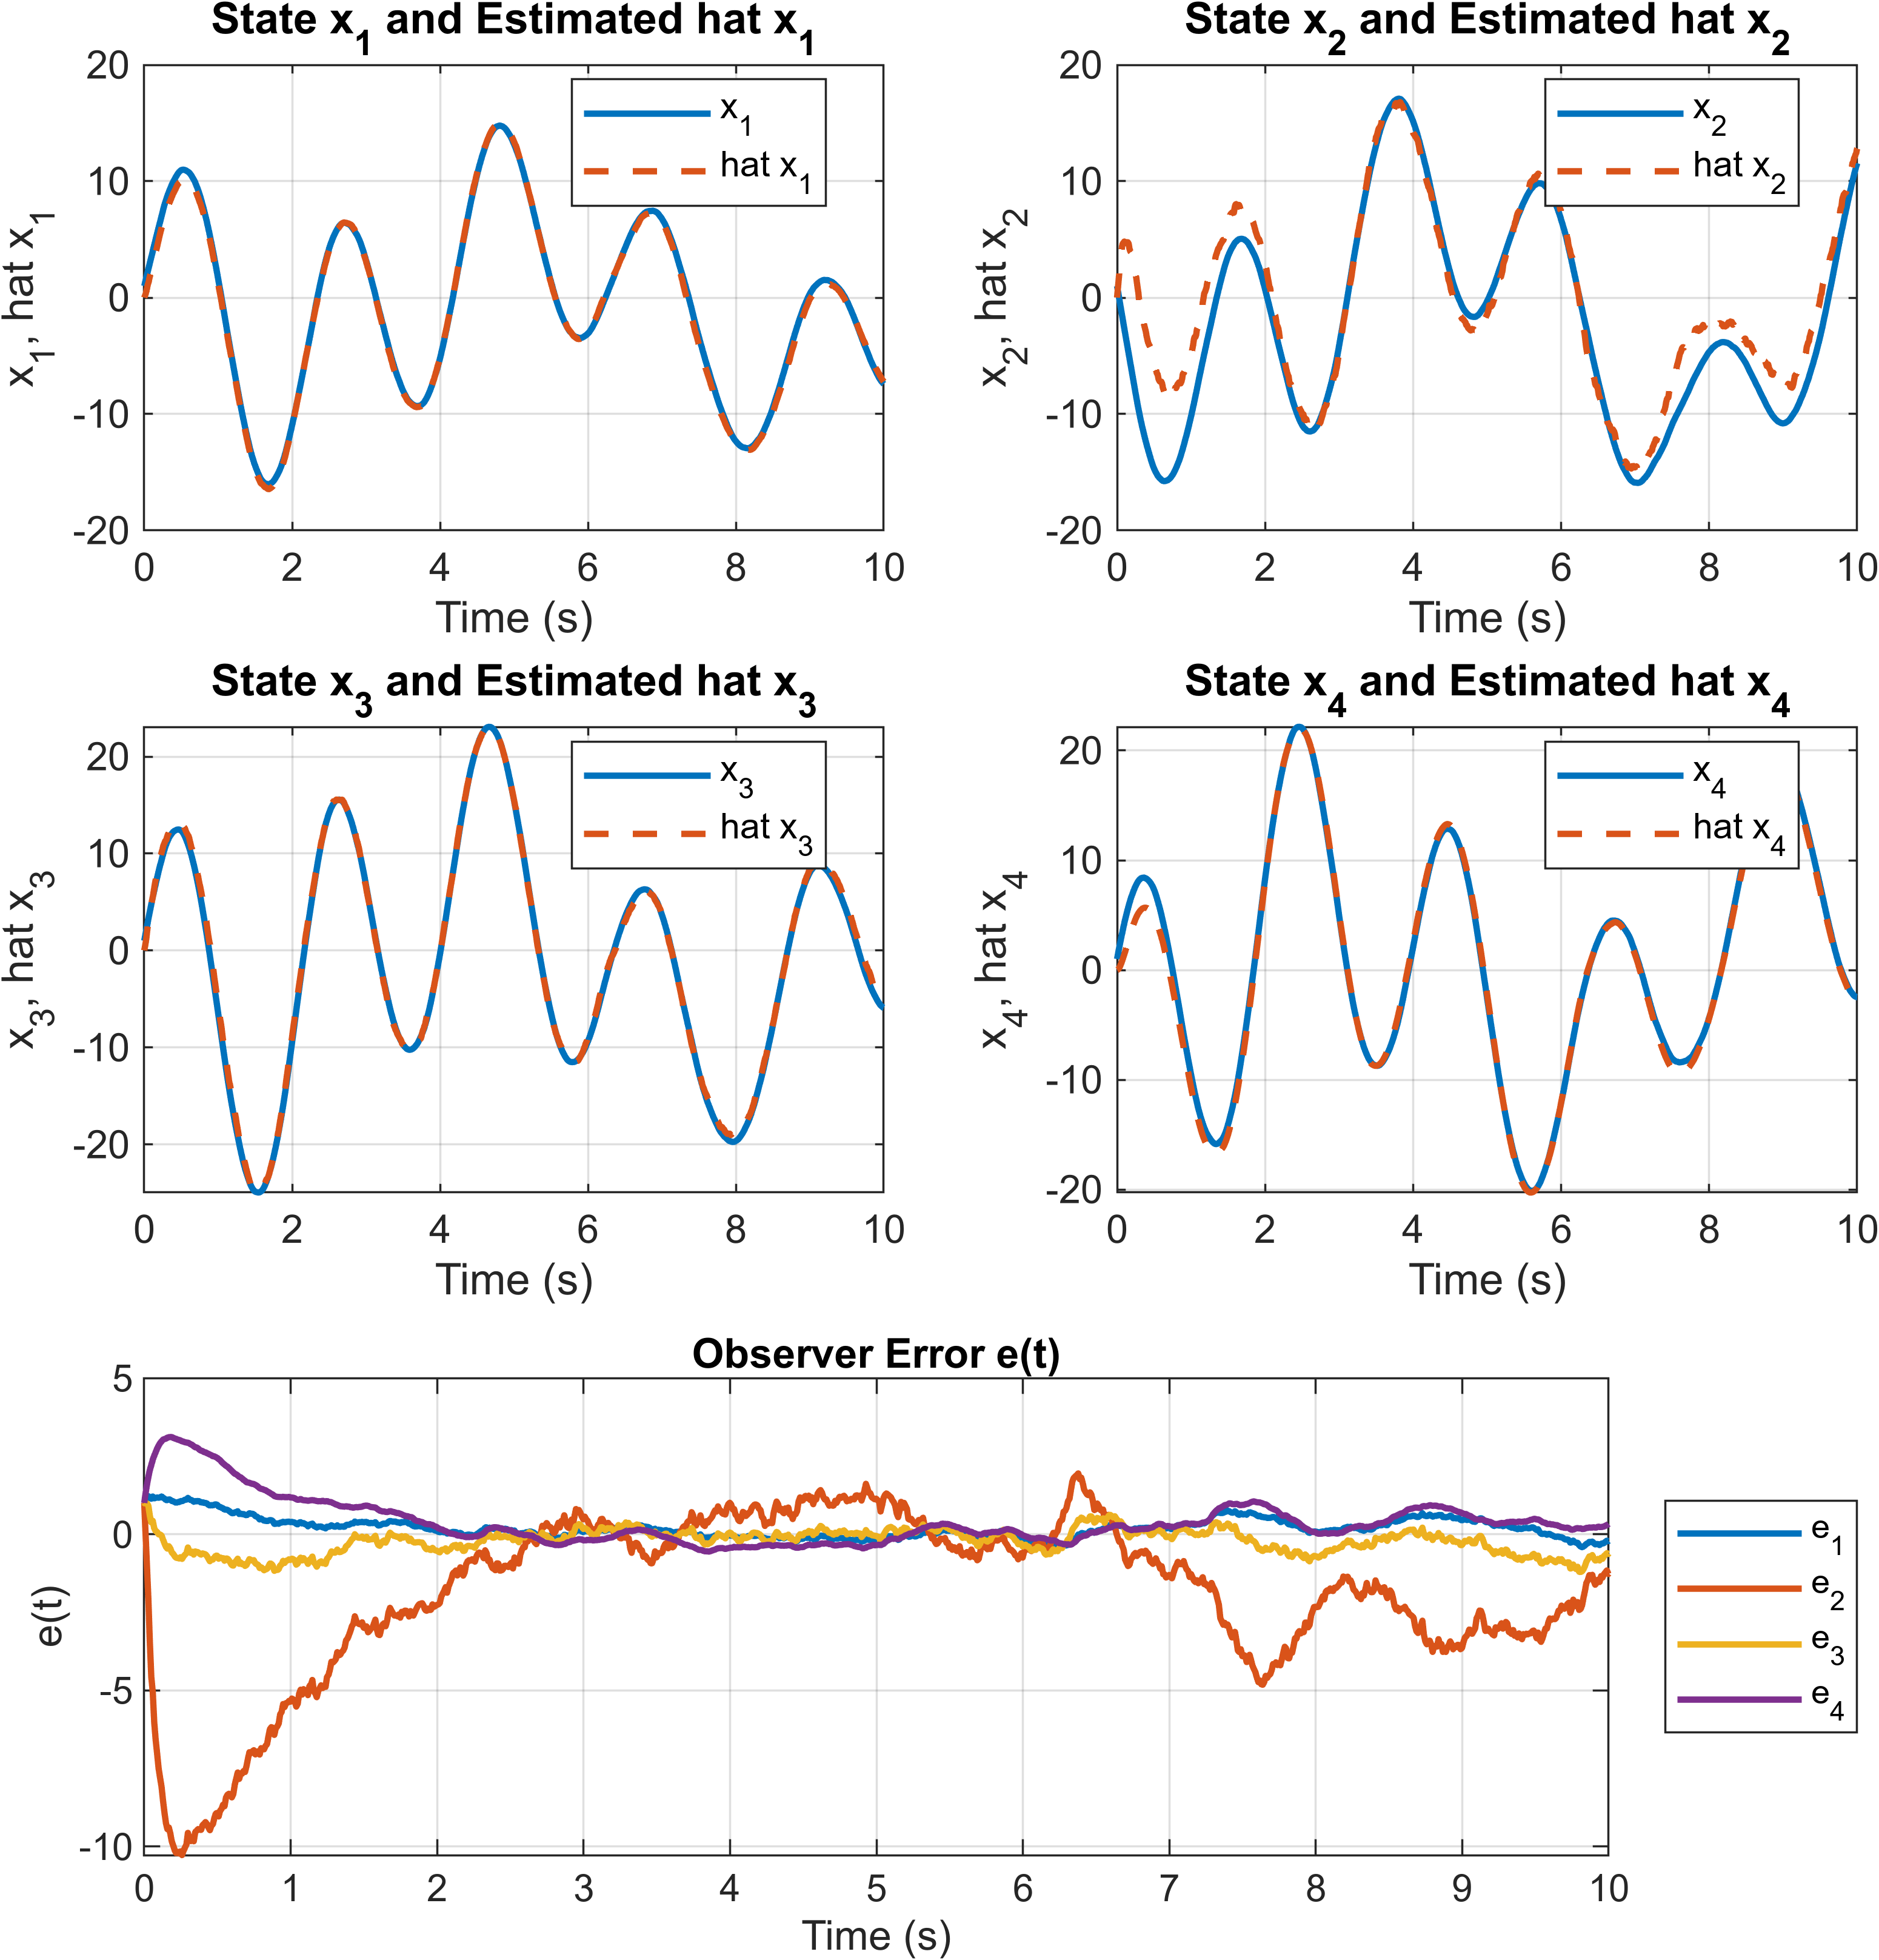
\includegraphics[width=1\linewidth]{figs/2_sim4.png}
    \caption{Моделирование замкнутой системы \eqref{eq:sys2} для пары $(\alpha Q,\ \alpha  R )$}
    \label{fig:sys2sim4}
\end{figure}

\newpage\subsection{Выводы}

Рассмотрев результаты моделирования для различных пар $(Q, R)$, можно сделать 
следующие выводы:
\begin{enumerate}
    \item Увеличение матрицы $Q$ (переход от $(Q, R)$ к $(\alpha Q, R)$) 
    приводит к увеличению шумов в состоянии наблюдателя. Таким образом,
    наблюдатель "верит", что шума почти нет.
    \item Увеличение матрицы $R$ (переход от $(Q, R)$ к $(Q, \alpha R)$) 
    приводит отсутствию каких либо шумов в состоянии наблюдателя, но ошибка
    серьезно увеличилась. Таким образом, наблюдатель "верит", что шума очень много и 
    не доверяет показаниям выхода.
    \item Увеличение обеих матриц $Q$ и $R$ (переход от $(Q, R)$ к $(\alpha Q, \alpha R)$) 
    не оказывает влияния на поведение наблюдателя, 
    что говорит о важности соотношения матриц $Q$ и $R$, а не их абсолютных значений.
\end{enumerate}
Таким образом, увеличение элементов $Q$ делает наблюдатель более 
"доверчивым" выходу, что увеличиваем восприимчивость к шумам, 
а увеличение элементов $R$ — менее доверчивым выходу, что уменьшает влияние шумов,
но увеличивает ошибку наблюдателя.





\newpage \section{Синтез LQG}
\subsection{Система}
Рассмотрим систему
\begin{equation}
    \label{eq:sys3}
    \begin{cases}
        \dot x=Ax+Bu+f\\
        y=Cx+Du+\xi
    \end{cases},\quad
    x(0)=\begin{bmatrix}
        1&1&1&1
    \end{bmatrix}^T,
\end{equation}
где
\begin{equation*}
    A=\begin{bmatrix}
        5 & -5 & -9 & 3 \\
        -5 & 5 & -3 & 9 \\
        -9 & -3 & 5 & 5 \\
        3 & 9 & 5 & 5
    \end{bmatrix},\quad
    B=\begin{bmatrix}
        2 & 0 \\
        6 & 0 \\
        6 & 0 \\
        2 & 0
    \end{bmatrix},\quad
    C=\begin{bmatrix}
        1 & -1 & 1 & 1 \\
        1 & 3 & -1 & 3
    \end{bmatrix},\quad
    D=\begin{bmatrix}
        0 & 2 \\
        0 & 1
    \end{bmatrix},
\end{equation*}
\begin{equation*}
    f(t)=\begin{bmatrix}
        0.1cos(0.5t) & 0.1cos(t) & 0.1cos(0.5t) & 0.1cos(t)
    \end{bmatrix}^T,\quad 
    \xi(t)=\begin{bmatrix}
        0.2sin(2t) & 0.2sin(5t)
    \end{bmatrix}^T.
\end{equation*}
Проверим систему на стабилизируемость и обнаруживаемость.
Составим матрицу управляемости:
\begin{equation*}
    U=\begin{bmatrix}
        2   & 0   & -68   & 0   & -176   & 0   & -15680   & 0 \\
        6   & 0   & 20    & 0   & 1328   & 0   & 8768     & 0 \\
        6   & 0   & 4     & 0   & 1072   & 0   & 5440     & 0 \\
        2   & 0   & 100   & 0   & 496    & 0   & 19264    & 0
    \end{bmatrix},
\end{equation*}
она имеет полный ранг, значит система управляемая и, как следствие, стабилизируемая.
Система имеем следующие собственные числа:
\begin{equation*}
    \sigma(A)=\{-12,\ 4, 12,\ 16\}.
\end{equation*}
Для проверки обнаруживаемости составим матрицы Хаутуса:
\begin{equation*}
    H_1 = \begin{bmatrix}
        -12 I - A \\ C
    \end{bmatrix} =
    \begin{bmatrix}
        -17 & 5  & 9  & -3 \\
         5  & -17 & 3  & -9 \\
         9  & 3  & -17 & -5 \\
        -3  & -9 & -5  & -17 \\
         1  & -1 & 1   & 1 \\
         1  & 3  & -1  & 3
    \end{bmatrix},\quad
    \text{rank}(H_1) = 3,
\end{equation*}
\begin{equation*}
    H_2 = \begin{bmatrix}
    4 I - A \\ C
    \end{bmatrix} =
    \begin{bmatrix}
        -1 & 5 & 9 & -3 \\
         5 & -1 & 3 & -9 \\
         9 & 3 & -1 & -5 \\
        -3 & -9 & -5 & -1 \\
         1 & -1 & 1 & 1 \\
         1 & 3 & -1 & 3   
        \end{bmatrix},\quad
    \text{rank}(H_2) = 4,
\end{equation*}
\begin{equation*}
    H_3 = \begin{bmatrix}
    12 I - A \\ C
    \end{bmatrix} =
    \begin{bmatrix}
        7 & 5 & 9 & -3 \\
        5 & 7 & 3 & -9 \\
        9 & 3 & 7 & -5 \\
        -3 & -9 & -5 & 7 \\
        1 & -1 & 1 & 1 \\
        1 & 3 & -1 & 3   
    \end{bmatrix},\quad
    \text{rank}(H_3) = 4,
\end{equation*}
\begin{equation*}
    H_4 = \begin{bmatrix}
    16 I - A \\ C
    \end{bmatrix} =
    \begin{bmatrix}
        11 & 5  & 9  & -3 \\
         5 & 11 & 3  & -9 \\
         9 & 3  & 11 & -5 \\
        -3 & -9 & -5 & 11 \\
         1 & -1 & 1  & 1  \\
         1 & 3  & -1 & 3     
        \end{bmatrix},\quad
    \text{rank}(H_4) = 4,
\end{equation*}
как видно, только собственное число $-12$ ненаблюдаемо, и так как оно
отрицательное, то система обнаруживаема. Имеет смысл делать регулятор и наблюдатель.
Построим схему моделирования системы \eqref{eq:sys3} с регулятором $u=K\hat x$ и 
наблюдателем состояния, см. \autoref{fig:sys3}.
\begin{figure}[H]
    \centering
    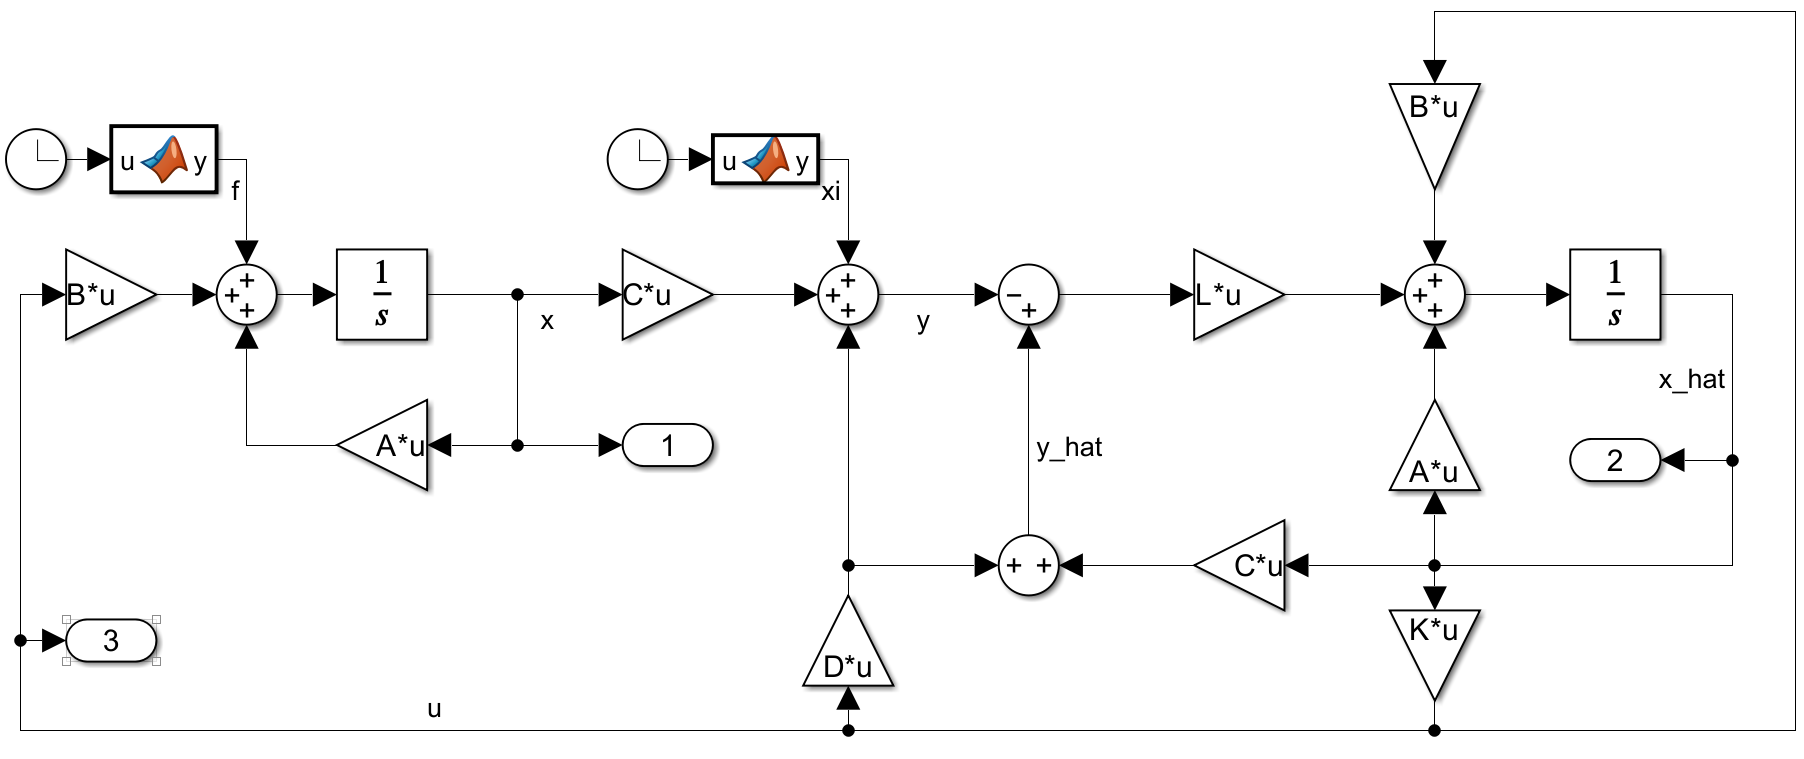
\includegraphics[width=1\linewidth]{figs/3_slx.png}
    \caption{Схема моделирования системы \eqref{eq:sys3} с регулятором и наблюдателем}
    \label{fig:sys3}
\end{figure}
\noindent Зададимся значениями пар матриц $(Q_K,\ R_K)$ для регулятора:
\begin{equation*}
    Q_K=\begin{bmatrix}
        10 & 0 & 0 & 0\\
        0 & 10 & 0 & 0\\
        0 & 0 & 10 & 0\\
        0 & 0 & 0 & 10
    \end{bmatrix},\quad
    R_K=\begin{bmatrix}
        1 & 0 \\
        0 & 1
    \end{bmatrix},
\end{equation*}
и $(Q_L,\ R_L)$ для наблюдателя:
\begin{equation*}
    Q_L=\begin{bmatrix}
        1 & 0 & 0 & 0\\
        0 & 1 & 0 & 0\\
        0 & 0 & 1 & 0\\
        0 & 0 & 0 & 1
    \end{bmatrix},\quad
    R_L=\begin{bmatrix}
        2 & 0 \\
        0 & 2
    \end{bmatrix}
\end{equation*}

\subsection{Синтез регулятора и наблюдателя}
Синтезируем матрицу регулятора $K$, используя решение соответствующего
матричного уравнения Риккати \eqref{eq:ric1}:
\begin{equation*}
    K=\begin{bmatrix}
        186.0102 & 112.1506 & -215.4595 & 82.7013 \\
        0        & 0        & 0         & 0
    \end{bmatrix}.
\end{equation*}
Синтезируем матрицу наблюдателя $L$, используя решение соответствующего
матричного уравнения Риккати \eqref{eq:ric2}:
\begin{equation*}
    L=\begin{bmatrix}
        -2.0607 &  78.0975 \\
         2.0607 & -35.4308 \\
        -2.0607 & -78.0975 \\
        -2.0607 & -35.4308
    \end{bmatrix}.
\end{equation*}

\subsection{Компьютерное моделирование}
Выполним компьютерное моделирование системы \eqref{eq:sys3} с регулятором и наблюдателем
с нулевыми начальными устовиями наблюдателя. Графики формумируемого управления $u(t)$,
сравнения $x(t)$ и $\hat x(t)$, а также ошибки наблюдателя $e(t)=\hat x(t)-x(t)$
приведены на \autoref{fig:sys3sim}.

\begin{figure}[H]
    \centering
    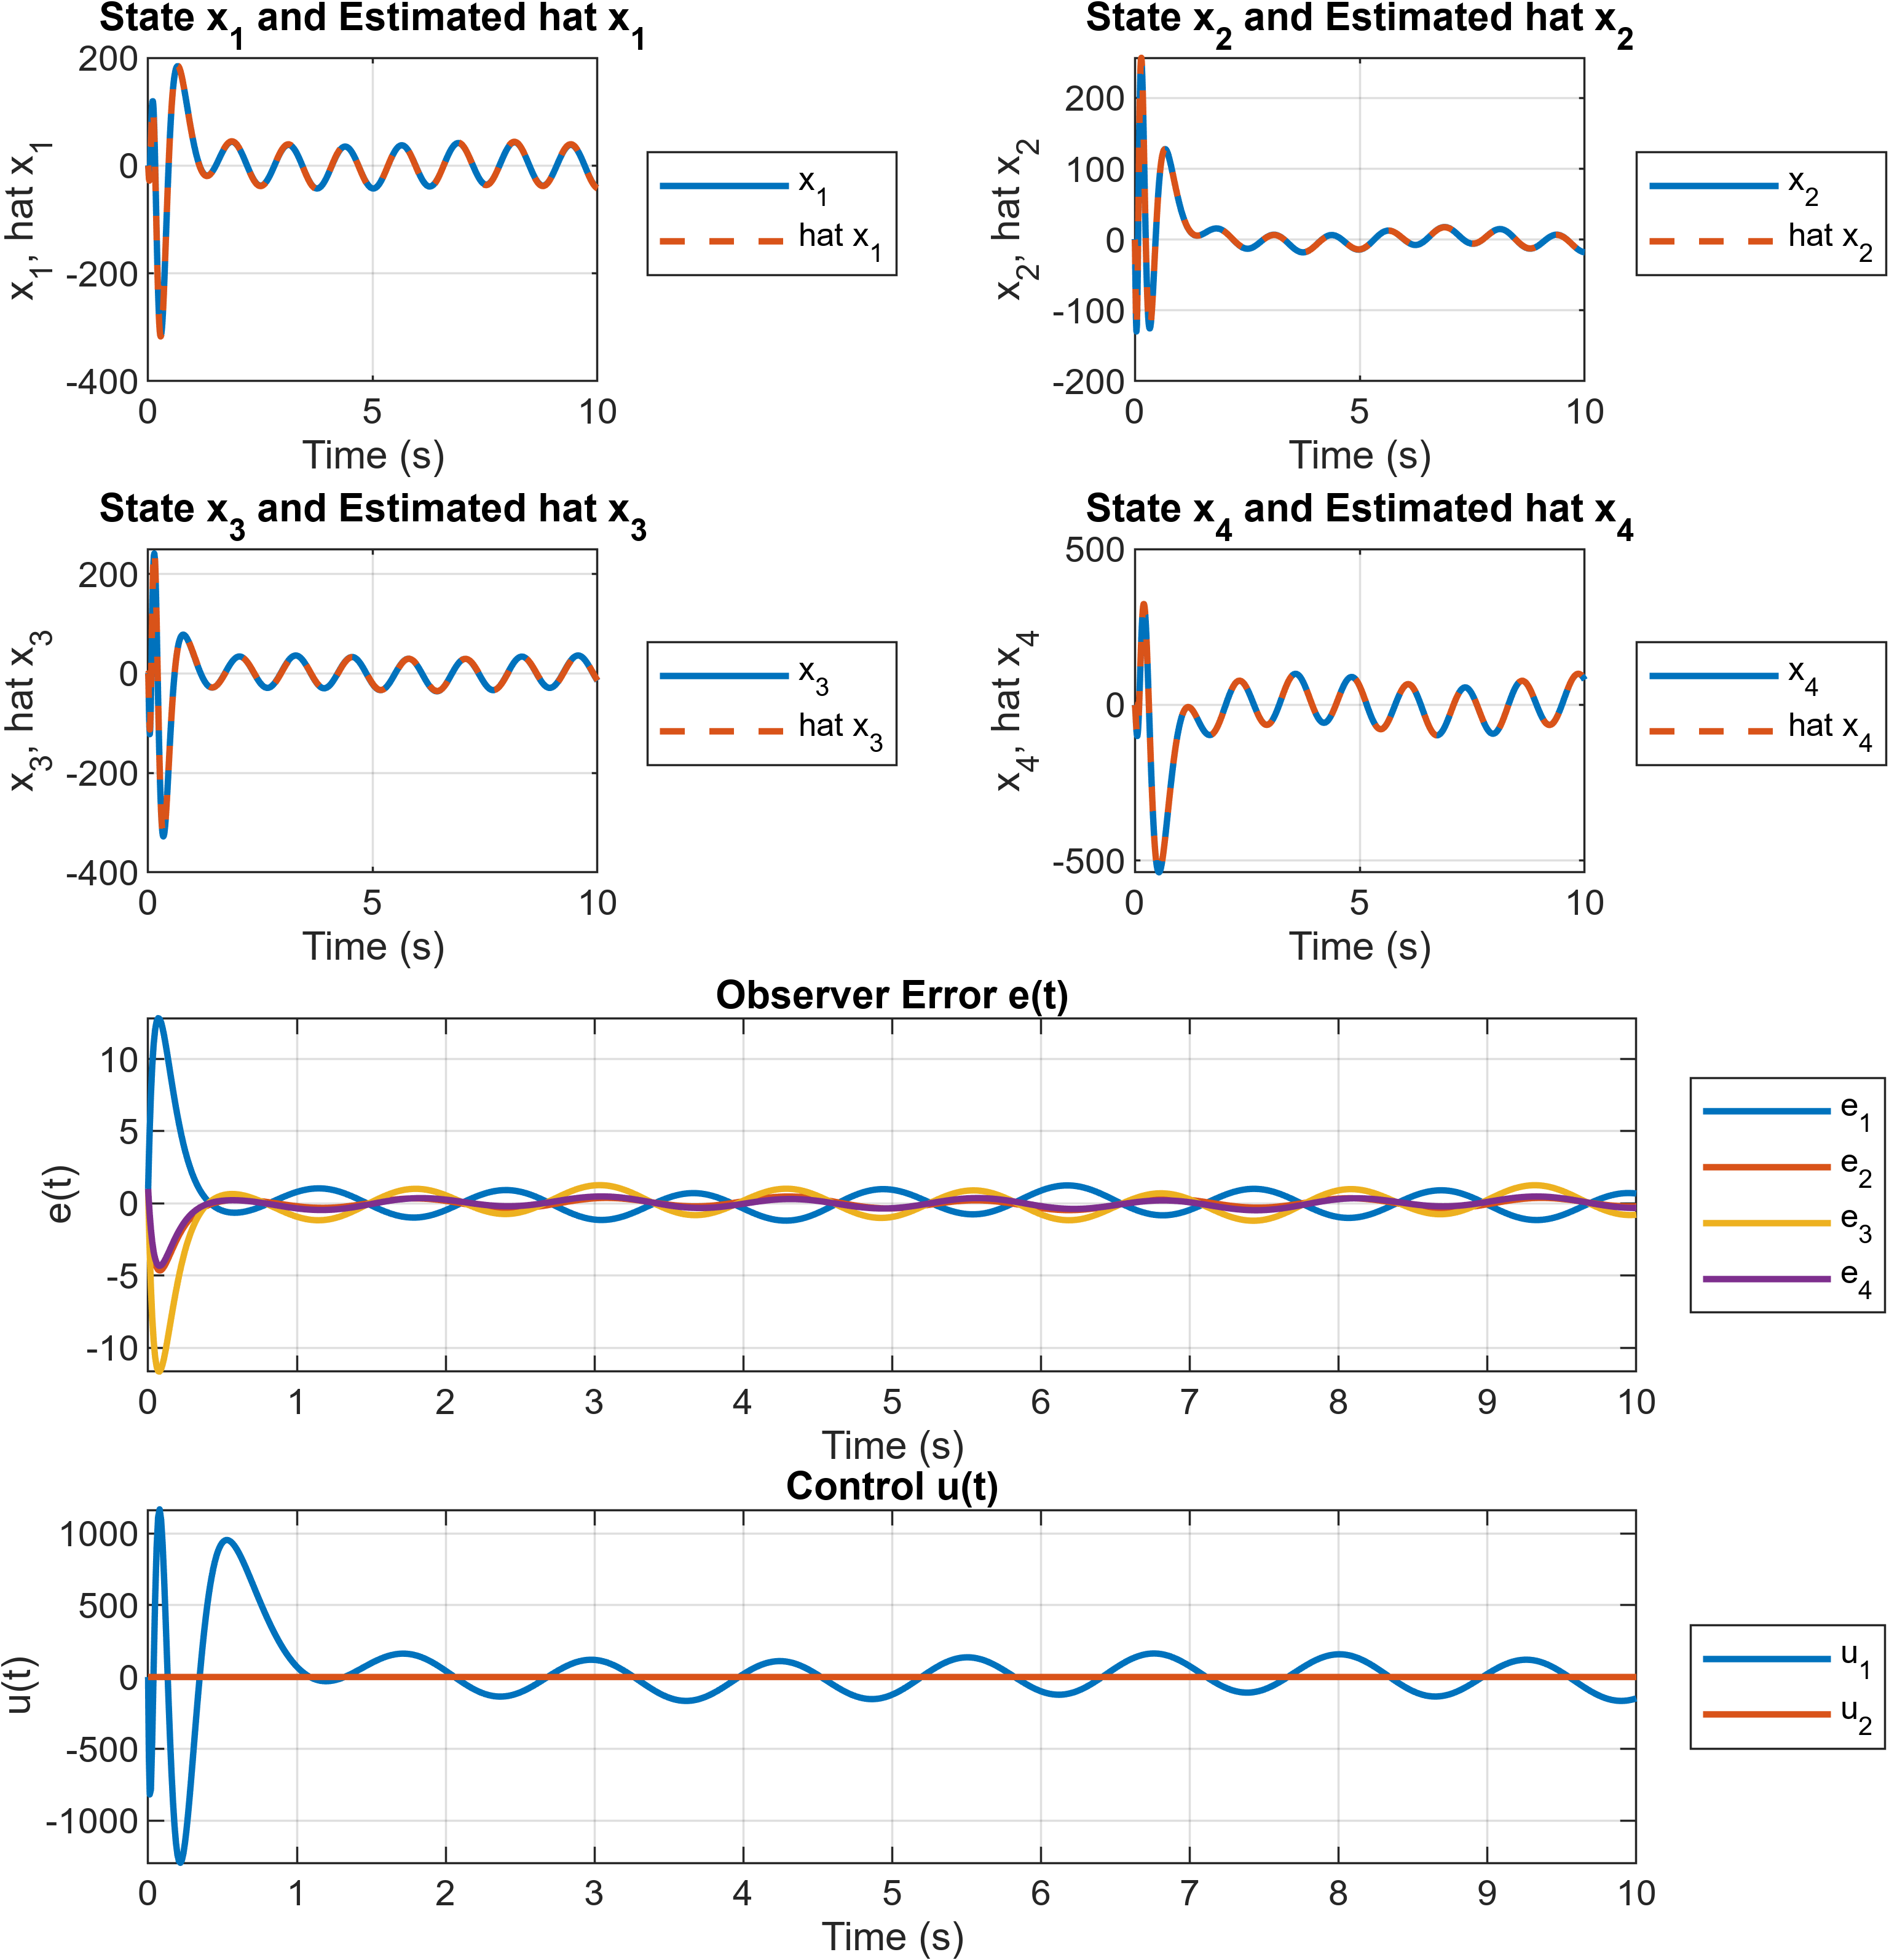
\includegraphics[width=1\linewidth]{figs/3_sim.png}
    \caption{Моделирование замкнутой системы \eqref{eq:sys3} с регулятором и наблюдателем}
    \label{fig:sys3sim}
\end{figure}

\newpage\subsection{Выводы}
Рассмотрев результаты моделирования, можно увидеть, что 
система пытается стабилизироваться, но не может полностью погасить внешнее
грамоническое возмущение. 
Наблюдатель также оценивает состояние системы с небольшой колеблющейся ощибкой.
Выбором матриц $Q_K$ и $R_K$ была дана задача "не жалеть" управления и побыстрее
свести состояние в ноль, что видно на графике управления.


\section{Заключение}
В работе исследованы LQR, фильтр Калмана и LQG (LQR + LQE). Проведен анализ влияния 
матриц $Q$ и $R$ как в регуляторе так и в наблюдателе на систему. 
Было показано, что соотношение матриц $Q$ и $R$ играет ключевую роль в поведении системы. 
Кроме того, синтез LQG-регулятора продемонстрировал возможность объединения 
оптимального управления и наблюдения для стабилизации системы в условиях 
внешних возмущений и шумов. Полность подавить гармонические или случайные 
возмущения не получилось.